
% Encoding: UTF-8
%%%%%%%%%%%%%%%%%%%%%%%%%%%%%%%%%%%%%%%%%%%%%%%%%%%%%%%%%%%%%%%%%%%%%%%%%%%%%%%

%%%%%%%%%%%%%%%%%%%%%%%%%%%%%%%%%%%%%%%%%%%%%%%%%%%%%%%%%%%%%%%%%%%%%%%%%%%%%%%
% $Id: slides.tex 17 2011-02-10 15:21:56Z klugeflo $
%%%%%%%%%%%%%%%%%%%%%%%%%%%%%%%%%%%%%%%%%%%%%%%%%%%%%%%%%%%%%%%%%%%%%%%%%%%%%%%

%%%%%%%%%%%%%%%%%%%%%%%%%%%%%%%%%%%%%%%%%%%%%%%%%%%%%%%%%%%%%%%%%%%%%%%%%%%%%%%
%%
%% Vorlage fuer LaTeX-Beamer
%% gemaess dem Corporate Design der Uni Augsburg
%%
%%%%%%%%%%%%%%%%%%%%%%%%%%%%%%%%%%%%%%%%%%%%%%%%%%%%%%%%%%%%%%%%%%%%%%%%%%%%%%%
%%
%% Changelog:
%%
%% 11/02/10 (FAK) Start
%%
%%%%%%%%%%%%%%%%%%%%%%%%%%%%%%%%%%%%%%%%%%%%%%%%%%%%%%%%%%%%%%%%%%%%%%%%%%%%%%%


%%%%%%%%%%%%%%%%%%%%%%%%%%%%%%%%%%%%%%%%%%%%%%%%%%%%%%%%%%%%%%%%%%%%%%%%%%%%%%%

\documentclass[xcolor=pdftex,dvipsnames,table]{beamer}
\setbeamertemplate{navigation symbols}{}%remove navigation symbols
%%%%%%%%%%%%%%%%%%%%%%%%%%%%%%%%%%%%%%%%%%%%%%%%%%%%%%%%%%%%%%%%%%%%%%%%%%%%%%%

% Language settings
% IMPORTANT: If you change the language settings, make sure to run
% cleantex prior to any latex/pdflatex to remove all .aux files, else
% latex might fail!
\usepackage[english]{babel}
%\usepackage[german]{babel}

\usepackage{pdfpages}
\usepackage{graphicx}
\usepackage{tikz}
\usepackage[utf8]{inputenc}
%\usepackage{mathptmx}

\usepackage{listings}

%%%%%%%%%%%%%%%%%%%%%%%%%%%%%%%%%%%%%%%%%%%%%%%%%%%%%%%%%%%%%%%%%%%%%%%%%%%%%%%

%\usetheme{fai}

% IMPORTANT/TODO: currently only PDF graphic files should be used, PNG
% or JPEG may harm the Adobe Reader colour palette and result in
% strange display colours.
%\DeclareGraphicsExtensions{.pdf}

\graphicspath{{./img/}}

%%%%%%%%%%%%%%%%%%%%%%%%%%%%%%%%%%%%%%%%%%%%%%%%%%%%%%%%%%%%%%%%%%%%%%%%%%%%%%%
%% Presentation main settings
%%%%%%%%%%%%%%%%%%%%%%%%%%%%%%%%%%%%%%%%%%%%%%%%%%%%%%%%%%%%%%%%%%%%%%%%%%%%%%%

\title{Systemnahe Informatik}
\subtitle{Übungsgruppe Xeon Phi}
\author{Dominik Walter}
\date{Sommersemester 2018}


%%%%%%%%%%%%%%%%%%%%%%%%%%%%%%%%%%%%%%%%%%%%%%%%%%%%%%%%%%%%%%%%%%%%%%%%%%%%%%%
%% Main Document starts here
%%%%%%%%%%%%%%%%%%%%%%%%%%%%%%%%%%%%%%%%%%%%%%%%%%%%%%%%%%%%%%%%%%%%%%%%%%%%%%%



\begin{document}
	
	\begin{frame}
	\frametitle{\ }
	\titlepage
\end{frame}
%{
%\section{Titlepage}
%
%	\usebackgroundtemplate%
%	{%
%%	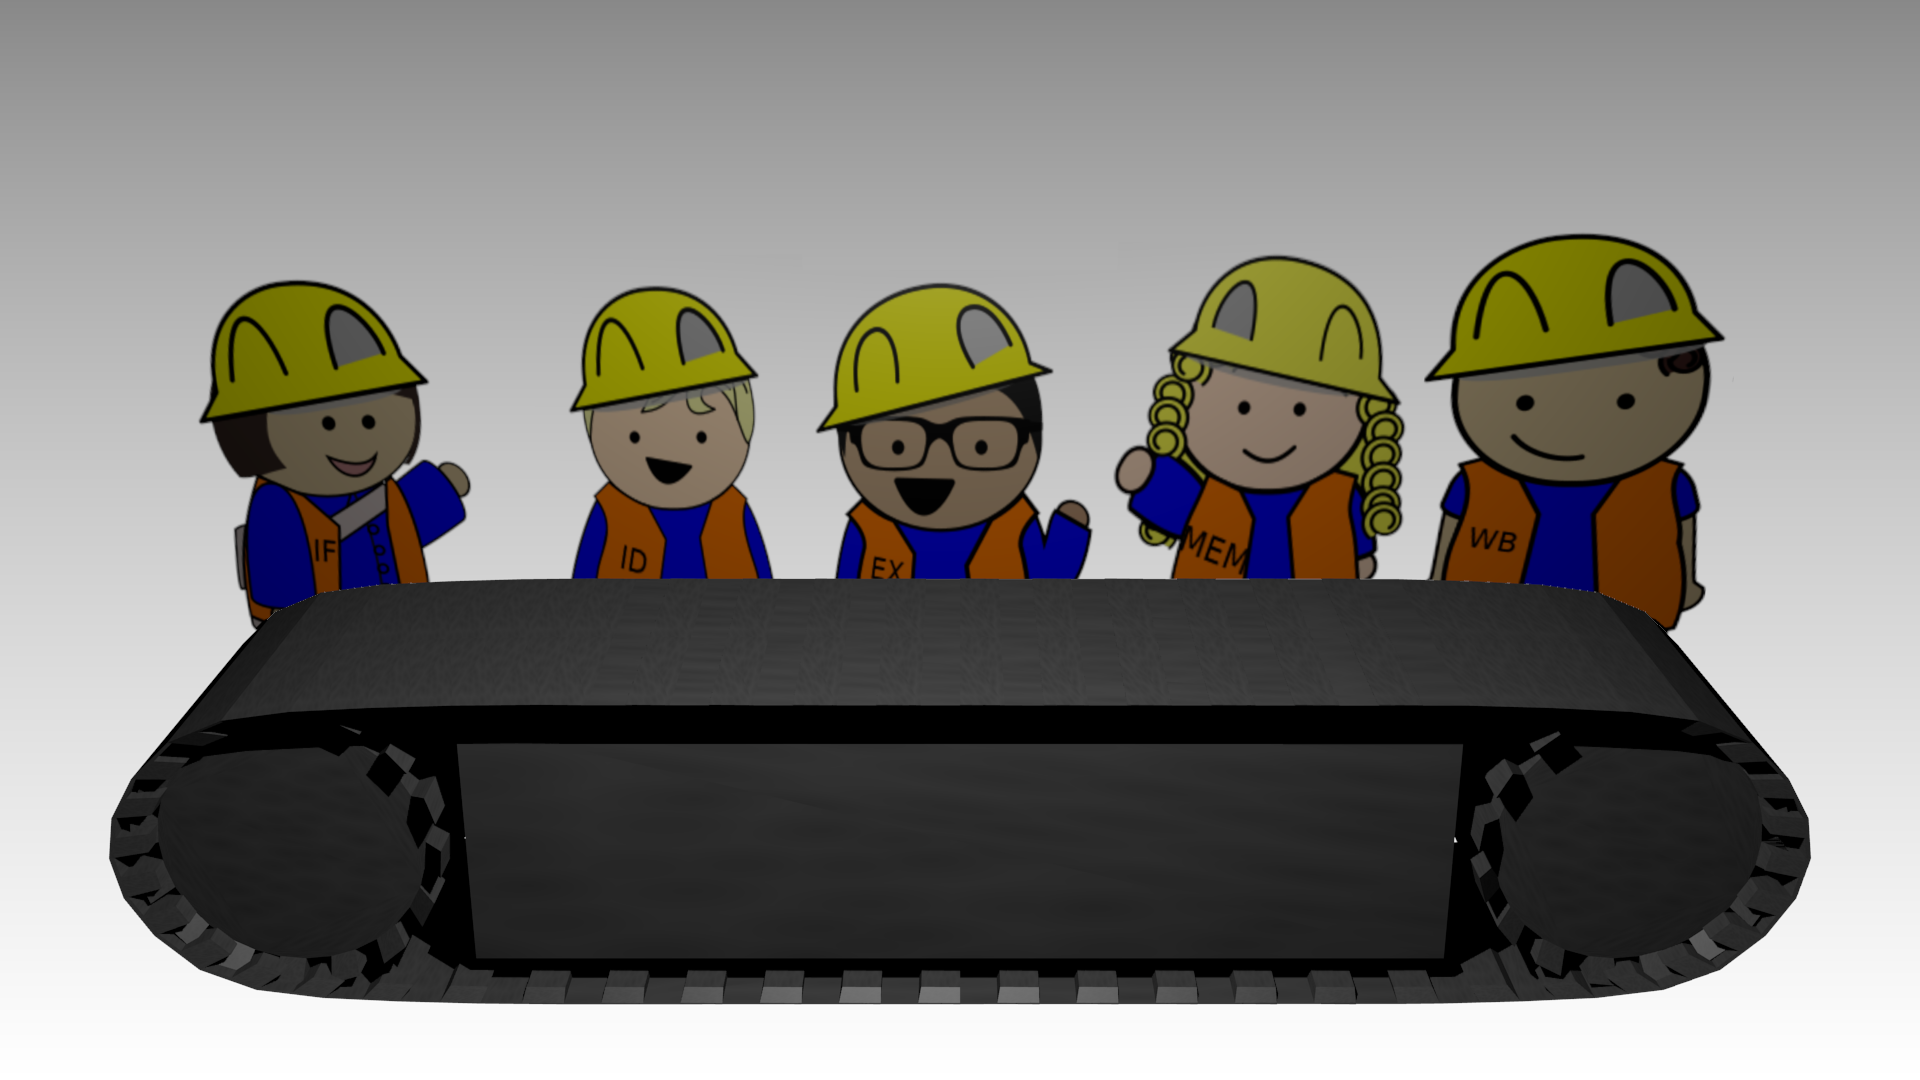
\includegraphics[width=\paperwidth,height=\paperheight]{final}%
%	}
%\begin{frame}
%%\phantom{empty}
%%\phantom{empty}
%%\phantom{empty}
%%\phantom{empty}
%%\phantom{empty}
%%\phantom{empty}
%%\phantom{empty}
%%\color{white}
%		\huge
%		\centering
%		\underline{RISCV-Pipeline}
%		\large
%		\\Systemnahe Informatik
%		\small
%		\\Übungsgruppe Xeon Phi
%		%Dominik Walter
%		
%		%08.02.2018
%
%
%\end{frame}
%
%}
%%%%%%%%%%%%%%%%%%%%%%%%%%%%%%%%%%%%%%%%%%%%%%%%%%%%%%%%%%%%%%%%%%%%%%%%%%%%%%%

%%%%%%%%%%%%%%%%%%%%%%%%%%%%%%%%%%%%%%%%%%%%%%%%%%%%%%%%%%%%%%%%%%%%%%%%%%%%%%%

\section{Allgemein}


%%=============================================================================

\begin{frame}[fragile]
\frametitle{Conditional Branch}
\centering
\begin{lstlisting}
0:	add t0, zero, 1
4:	add t1, zero, 1
8:	nop
12:	nop
16:	beq t0, t1, end
20:	add t2, zero, 3
24:	add t3, zero, 4
28:	add t4, zero, 5
32:	add t5, zero, 6
end:
36:	mul t0, t1, t2
\end{lstlisting}
\end{frame}

\begin{frame}
\frametitle{Conditional Branch | Takt 0}
\begin{picture}(0,0)
\put(0,-85){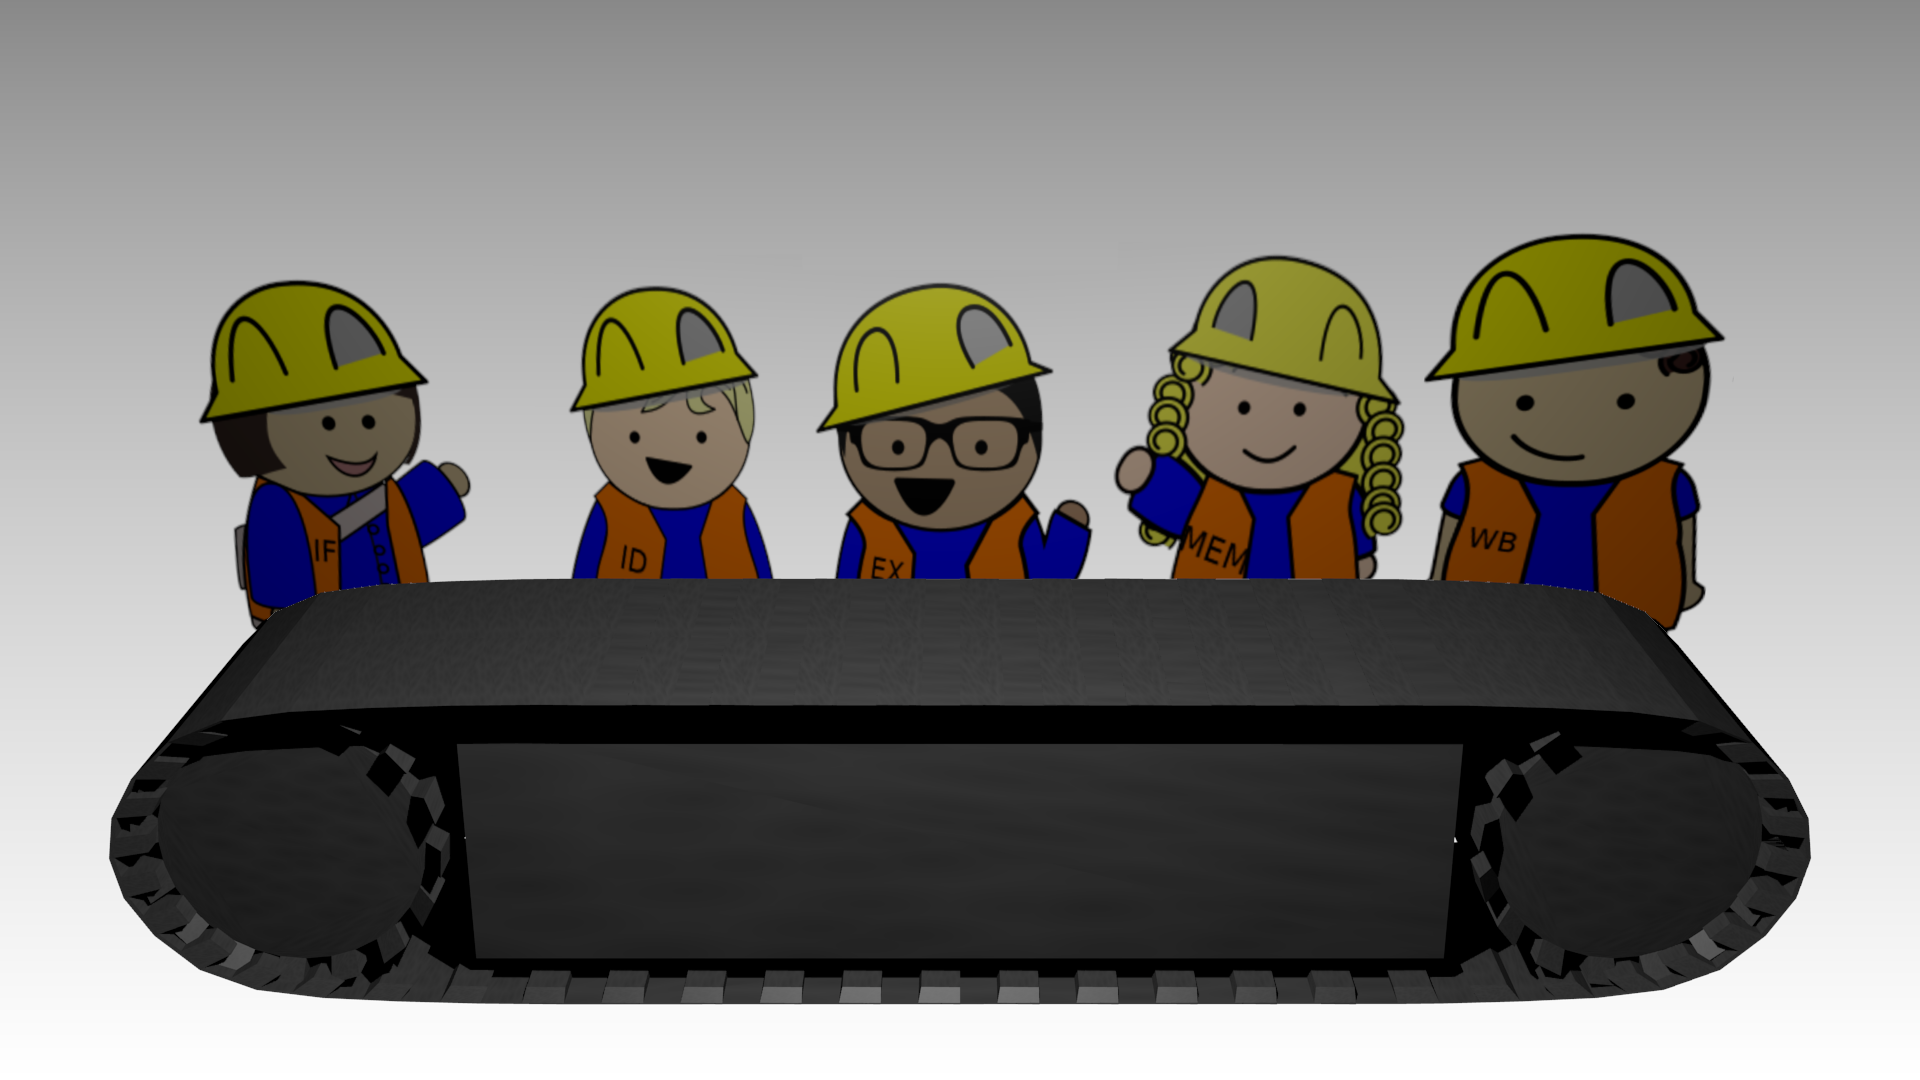
\includegraphics[width=1.0\textwidth]{final.png}}
%FETCH
\put(50,-12){\fontsize{5.5}{4}\selectfont\color{white}add t0, zero, 1}

%DECODE
\put(90,-12){\fontsize{5.5}{4}\selectfont\color{white}}
\put(90,-17){\fontsize{5.5}{4}\selectfont\color{white}}

%EXECUTE
\put(135,-12){\fontsize{5.5}{4}\selectfont\color{white}}
\put(135,-17){\fontsize{5.5}{4}\selectfont\color{white}}
\put(135,-22){\fontsize{5.5}{4}\selectfont\color{white}}

%MEMORY
\put(185,-12){\fontsize{5.5}{4}\selectfont\color{white}}
\put(185,-17){\fontsize{5.5}{4}\selectfont\color{white}}
\put(185,-22){\fontsize{5.5}{4}\selectfont\color{white}}

%WRITEBACK
\put(225,-12){\fontsize{5.5}{4}\selectfont\color{white}}
\put(225,-17){\fontsize{5.5}{4}\selectfont\color{white}}
\put(225,-22){\fontsize{5.5}{4}\selectfont\color{white}}

%REGISTERS
\put(80,-37){\fontsize{5.5}{4}\selectfont\color{white}zero = 0}
\put(80,-42){\fontsize{5.5}{4}\selectfont\color{white}ra = 0}
\put(80,-47){\fontsize{5.5}{4}\selectfont\color{white}sp = 0}
\put(80,-52){\fontsize{5.5}{4}\selectfont\color{white}pc = 0}
\put(80,-57){\fontsize{5.5}{4}\selectfont\color{white}t0 = 0}
\put(80,-62){\fontsize{5.5}{4}\selectfont\color{white}t1 = 0}

\put(110,-37){\fontsize{5.5}{4}\selectfont\color{white}t2 = 0}
\put(110,-42){\fontsize{5.5}{4}\selectfont\color{white}t3 = 0}
\put(110,-47){\fontsize{5.5}{4}\selectfont\color{white}t4 = 0}
\put(110,-52){\fontsize{5.5}{4}\selectfont\color{white}t5 = 0}
\put(110,-57){\fontsize{5.5}{4}\selectfont\color{white}t6 = 0}
\put(110,-62){\fontsize{5.5}{4}\selectfont\color{white}a0 = 0}

\put(140,-37){\fontsize{5.5}{4}\selectfont\color{white}a1 = 0}
\put(140,-42){\fontsize{5.5}{4}\selectfont\color{white}a2 = 0}
\put(140,-47){\fontsize{5.5}{4}\selectfont\color{white}a3 = 0}
\put(140,-52){\fontsize{5.5}{4}\selectfont\color{white}a4 = 0}
\put(140,-57){\fontsize{5.5}{4}\selectfont\color{white}a5 = 0}
\put(140,-62){\fontsize{5.5}{4}\selectfont\color{white}a6 = 0}

\put(170,-37){\fontsize{5.5}{4}\selectfont\color{white}a7 = 0}
\put(170,-42){\fontsize{5.5}{4}\selectfont\color{white}s1 = 0}
\put(170,-47){\fontsize{5.5}{4}\selectfont\color{white}s2 = 0}
\put(170,-52){\fontsize{5.5}{4}\selectfont\color{white}s3 = 0}
\put(170,-57){\fontsize{5.5}{4}\selectfont\color{white}s4 = 0}
\put(170,-62){\fontsize{5.5}{4}\selectfont\color{white}s5 = 0}

\put(200,-37){\fontsize{5.5}{4}\selectfont\color{white}s6 = 0}
\put(200,-42){\fontsize{5.5}{4}\selectfont\color{white}s7 = 0}
\put(200,-47){\fontsize{5.5}{4}\selectfont\color{white}s8 = 0}
\put(200,-52){\fontsize{5.5}{4}\selectfont\color{white}s9 = 0}
\put(200,-57){\fontsize{5.5}{4}\selectfont\color{white}s10 = 0}
\put(200,-62){\fontsize{5.5}{4}\selectfont\color{white}s11 = 0}

\end{picture}
\end{frame}


\begin{frame}
\frametitle{Conditional Branch | Takt 1}
\begin{picture}(0,0)
\put(0,-85){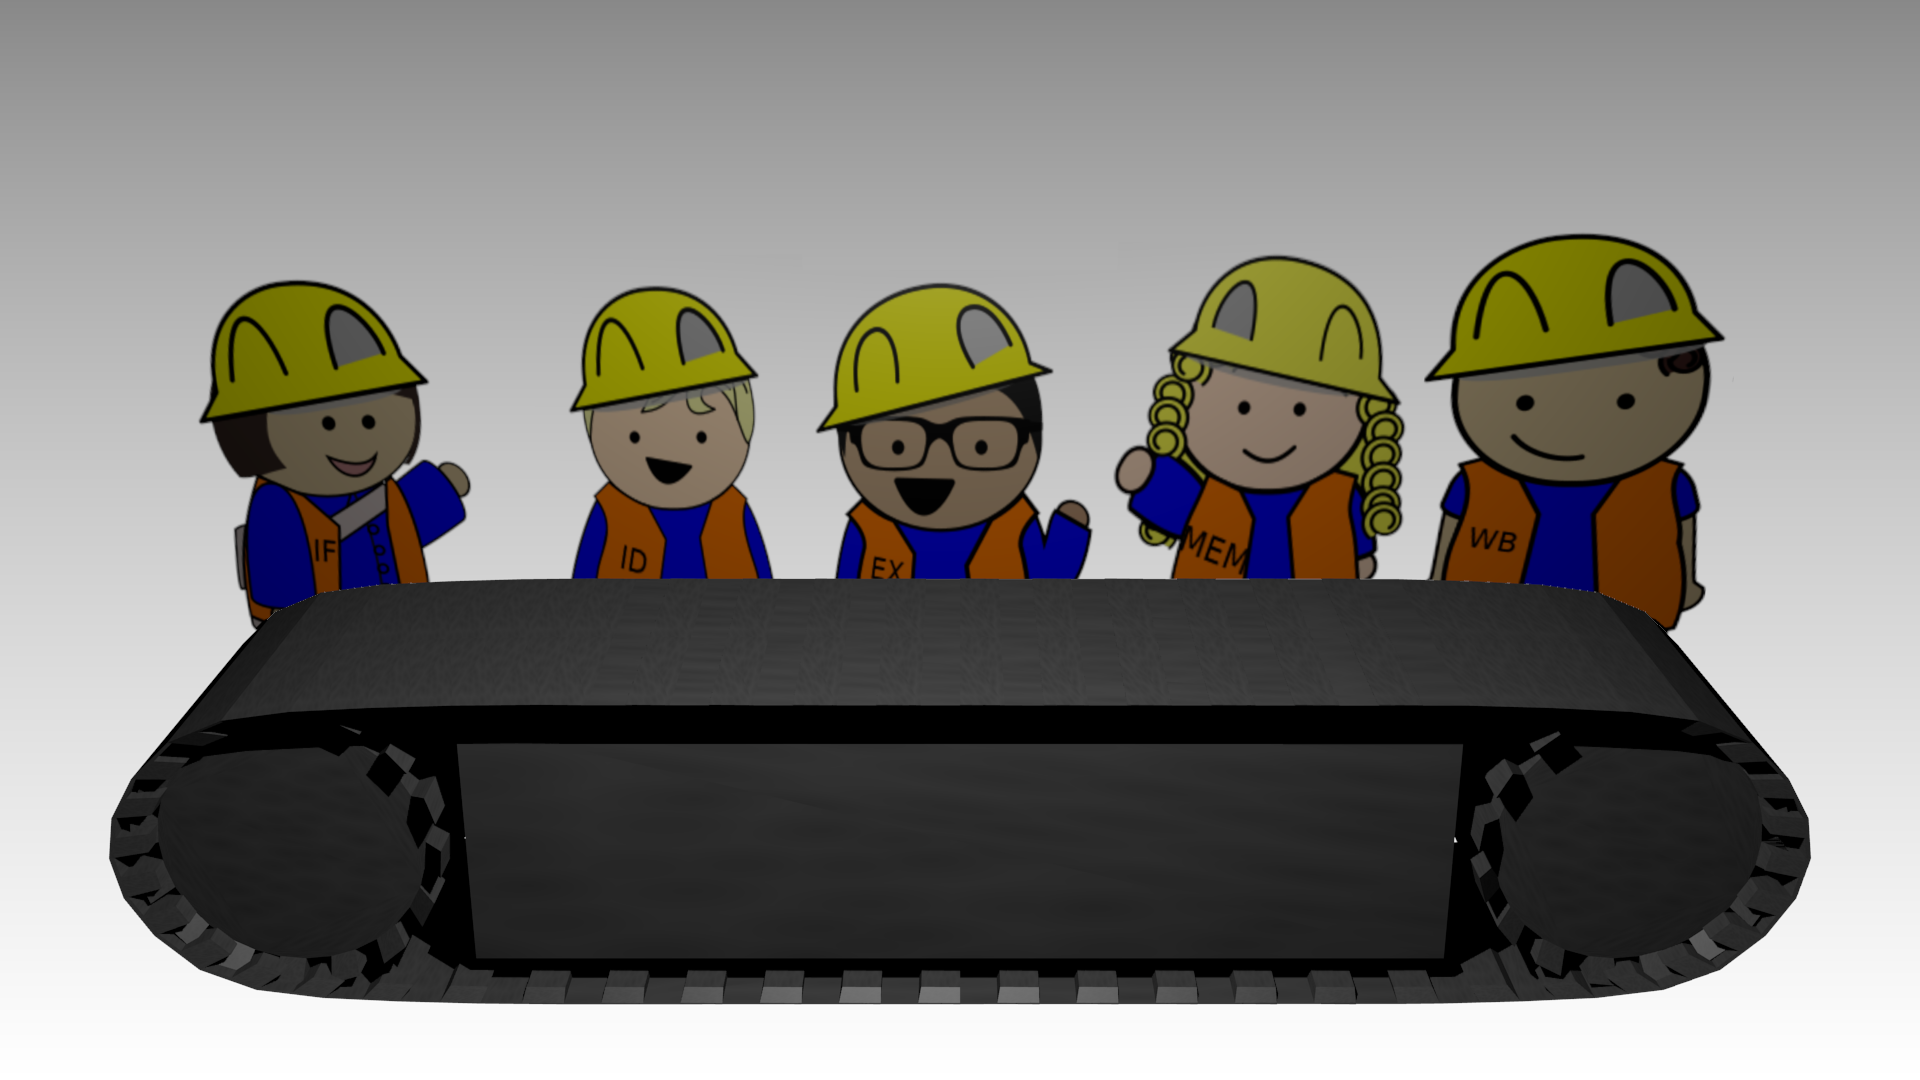
\includegraphics[width=1.0\textwidth]{final.png}}
%FETCH
\put(50,-12){\fontsize{5.5}{4}\selectfont\color{white}add t1, zero, 1}

%DECODE
\put(90,-12){\fontsize{5.5}{4}\selectfont\color{white}add t0, zero, 1}
\put(90,-17){\fontsize{5.5}{4}\selectfont\color{white}t0 = 0 + 1}

%EXECUTE
\put(135,-12){\fontsize{5.5}{4}\selectfont\color{white}}
\put(135,-17){\fontsize{5.5}{4}\selectfont\color{white}}
\put(135,-22){\fontsize{5.5}{4}\selectfont\color{white}}

%MEMORY
\put(185,-12){\fontsize{5.5}{4}\selectfont\color{white}}
\put(185,-17){\fontsize{5.5}{4}\selectfont\color{white}}
\put(185,-22){\fontsize{5.5}{4}\selectfont\color{white}}

%WRITEBACK
\put(225,-12){\fontsize{5.5}{4}\selectfont\color{white}}
\put(225,-17){\fontsize{5.5}{4}\selectfont\color{white}}
\put(225,-22){\fontsize{5.5}{4}\selectfont\color{white}}

%REGISTERS
\put(80,-37){\fontsize{5.5}{4}\selectfont\color{white}zero = 0}
\put(80,-42){\fontsize{5.5}{4}\selectfont\color{white}ra = 0}
\put(80,-47){\fontsize{5.5}{4}\selectfont\color{white}sp = 0}
\put(80,-52){\fontsize{5.5}{4}\selectfont\color{white}pc = 4}
\put(80,-57){\fontsize{5.5}{4}\selectfont\color{white}t0 = 0}
\put(80,-62){\fontsize{5.5}{4}\selectfont\color{white}t1 = 0}

\put(110,-37){\fontsize{5.5}{4}\selectfont\color{white}t2 = 0}
\put(110,-42){\fontsize{5.5}{4}\selectfont\color{white}t3 = 0}
\put(110,-47){\fontsize{5.5}{4}\selectfont\color{white}t4 = 0}
\put(110,-52){\fontsize{5.5}{4}\selectfont\color{white}t5 = 0}
\put(110,-57){\fontsize{5.5}{4}\selectfont\color{white}t6 = 0}
\put(110,-62){\fontsize{5.5}{4}\selectfont\color{white}a0 = 0}

\put(140,-37){\fontsize{5.5}{4}\selectfont\color{white}a1 = 0}
\put(140,-42){\fontsize{5.5}{4}\selectfont\color{white}a2 = 0}
\put(140,-47){\fontsize{5.5}{4}\selectfont\color{white}a3 = 0}
\put(140,-52){\fontsize{5.5}{4}\selectfont\color{white}a4 = 0}
\put(140,-57){\fontsize{5.5}{4}\selectfont\color{white}a5 = 0}
\put(140,-62){\fontsize{5.5}{4}\selectfont\color{white}a6 = 0}

\put(170,-37){\fontsize{5.5}{4}\selectfont\color{white}a7 = 0}
\put(170,-42){\fontsize{5.5}{4}\selectfont\color{white}s1 = 0}
\put(170,-47){\fontsize{5.5}{4}\selectfont\color{white}s2 = 0}
\put(170,-52){\fontsize{5.5}{4}\selectfont\color{white}s3 = 0}
\put(170,-57){\fontsize{5.5}{4}\selectfont\color{white}s4 = 0}
\put(170,-62){\fontsize{5.5}{4}\selectfont\color{white}s5 = 0}

\put(200,-37){\fontsize{5.5}{4}\selectfont\color{white}s6 = 0}
\put(200,-42){\fontsize{5.5}{4}\selectfont\color{white}s7 = 0}
\put(200,-47){\fontsize{5.5}{4}\selectfont\color{white}s8 = 0}
\put(200,-52){\fontsize{5.5}{4}\selectfont\color{white}s9 = 0}
\put(200,-57){\fontsize{5.5}{4}\selectfont\color{white}s10 = 0}
\put(200,-62){\fontsize{5.5}{4}\selectfont\color{white}s11 = 0}

\end{picture}
\end{frame}

\begin{frame}
\frametitle{Conditional Branch | Takt 2}
\begin{picture}(0,0)
\put(0,-85){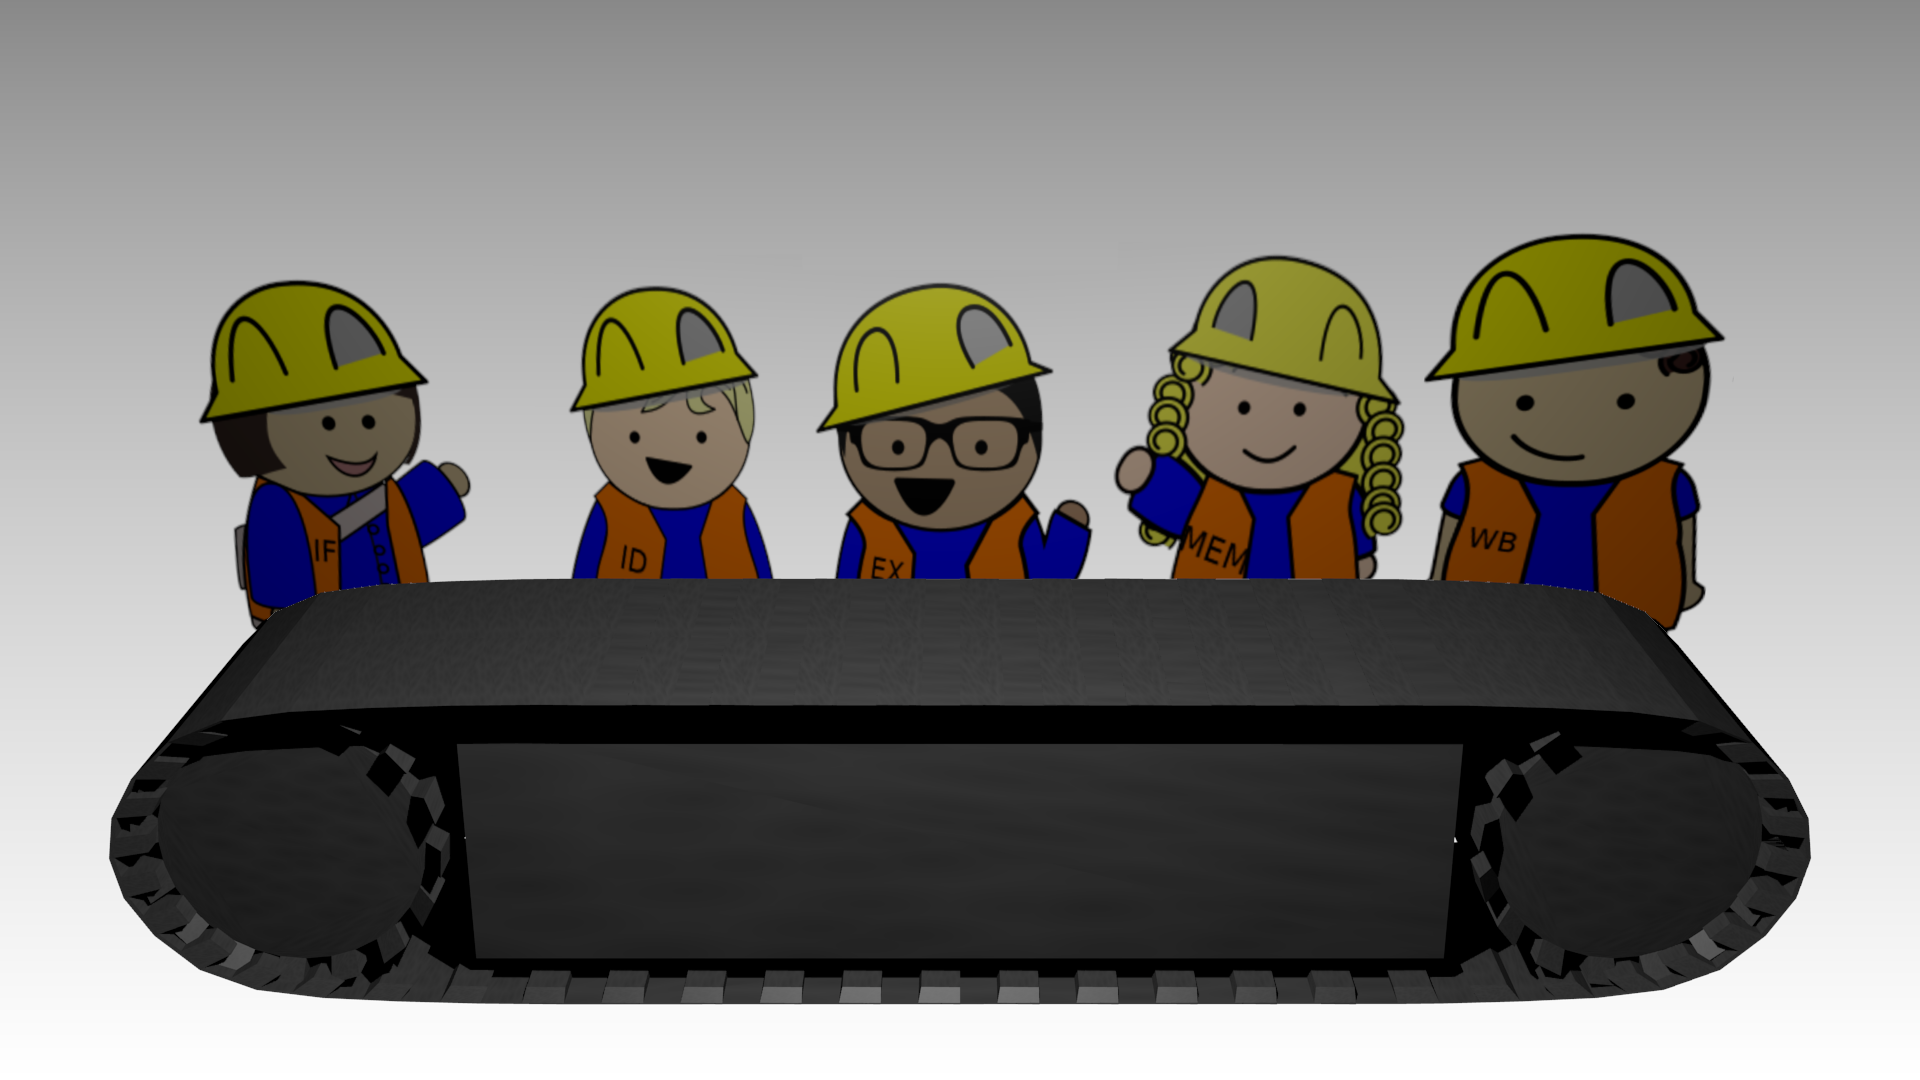
\includegraphics[width=1.0\textwidth]{final.png}}
%FETCH
\put(50,-12){\fontsize{5.5}{4}\selectfont\color{white}nop}

%DECODE
\put(90,-12){\fontsize{5.5}{4}\selectfont\color{white}add t1, zero, 1}
\put(90,-17){\fontsize{5.5}{4}\selectfont\color{white}t1 = 0 + 1}

%EXECUTE
\put(135,-12){\fontsize{5.5}{4}\selectfont\color{white}add t0, zero, 1}
\put(135,-17){\fontsize{5.5}{4}\selectfont\color{white}t0 = 0 + 1}
\put(135,-22){\fontsize{5.5}{4}\selectfont\color{white}t0 = 1}

%MEMORY
\put(185,-12){\fontsize{5.5}{4}\selectfont\color{white}}
\put(185,-17){\fontsize{5.5}{4}\selectfont\color{white}}
\put(185,-22){\fontsize{5.5}{4}\selectfont\color{white}}

%WRITEBACK
\put(225,-12){\fontsize{5.5}{4}\selectfont\color{white}}
\put(225,-17){\fontsize{5.5}{4}\selectfont\color{white}}
\put(225,-22){\fontsize{5.5}{4}\selectfont\color{white}}

%REGISTERS
\put(80,-37){\fontsize{5.5}{4}\selectfont\color{white}zero = 0}
\put(80,-42){\fontsize{5.5}{4}\selectfont\color{white}ra = 0}
\put(80,-47){\fontsize{5.5}{4}\selectfont\color{white}sp = 0}
\put(80,-52){\fontsize{5.5}{4}\selectfont\color{white}pc = 8}
\put(80,-57){\fontsize{5.5}{4}\selectfont\color{white}t0 = 0}
\put(80,-62){\fontsize{5.5}{4}\selectfont\color{white}t1 = 0}

\put(110,-37){\fontsize{5.5}{4}\selectfont\color{white}t2 = 0}
\put(110,-42){\fontsize{5.5}{4}\selectfont\color{white}t3 = 0}
\put(110,-47){\fontsize{5.5}{4}\selectfont\color{white}t4 = 0}
\put(110,-52){\fontsize{5.5}{4}\selectfont\color{white}t5 = 0}
\put(110,-57){\fontsize{5.5}{4}\selectfont\color{white}t6 = 0}
\put(110,-62){\fontsize{5.5}{4}\selectfont\color{white}a0 = 0}

\put(140,-37){\fontsize{5.5}{4}\selectfont\color{white}a1 = 0}
\put(140,-42){\fontsize{5.5}{4}\selectfont\color{white}a2 = 0}
\put(140,-47){\fontsize{5.5}{4}\selectfont\color{white}a3 = 0}
\put(140,-52){\fontsize{5.5}{4}\selectfont\color{white}a4 = 0}
\put(140,-57){\fontsize{5.5}{4}\selectfont\color{white}a5 = 0}
\put(140,-62){\fontsize{5.5}{4}\selectfont\color{white}a6 = 0}

\put(170,-37){\fontsize{5.5}{4}\selectfont\color{white}a7 = 0}
\put(170,-42){\fontsize{5.5}{4}\selectfont\color{white}s1 = 0}
\put(170,-47){\fontsize{5.5}{4}\selectfont\color{white}s2 = 0}
\put(170,-52){\fontsize{5.5}{4}\selectfont\color{white}s3 = 0}
\put(170,-57){\fontsize{5.5}{4}\selectfont\color{white}s4 = 0}
\put(170,-62){\fontsize{5.5}{4}\selectfont\color{white}s5 = 0}

\put(200,-37){\fontsize{5.5}{4}\selectfont\color{white}s6 = 0}
\put(200,-42){\fontsize{5.5}{4}\selectfont\color{white}s7 = 0}
\put(200,-47){\fontsize{5.5}{4}\selectfont\color{white}s8 = 0}
\put(200,-52){\fontsize{5.5}{4}\selectfont\color{white}s9 = 0}
\put(200,-57){\fontsize{5.5}{4}\selectfont\color{white}s10 = 0}
\put(200,-62){\fontsize{5.5}{4}\selectfont\color{white}s11 = 0}

\end{picture}
\end{frame}


\begin{frame}
\frametitle{Conditional Branch | Takt 3}
\begin{picture}(0,0)
\put(0,-85){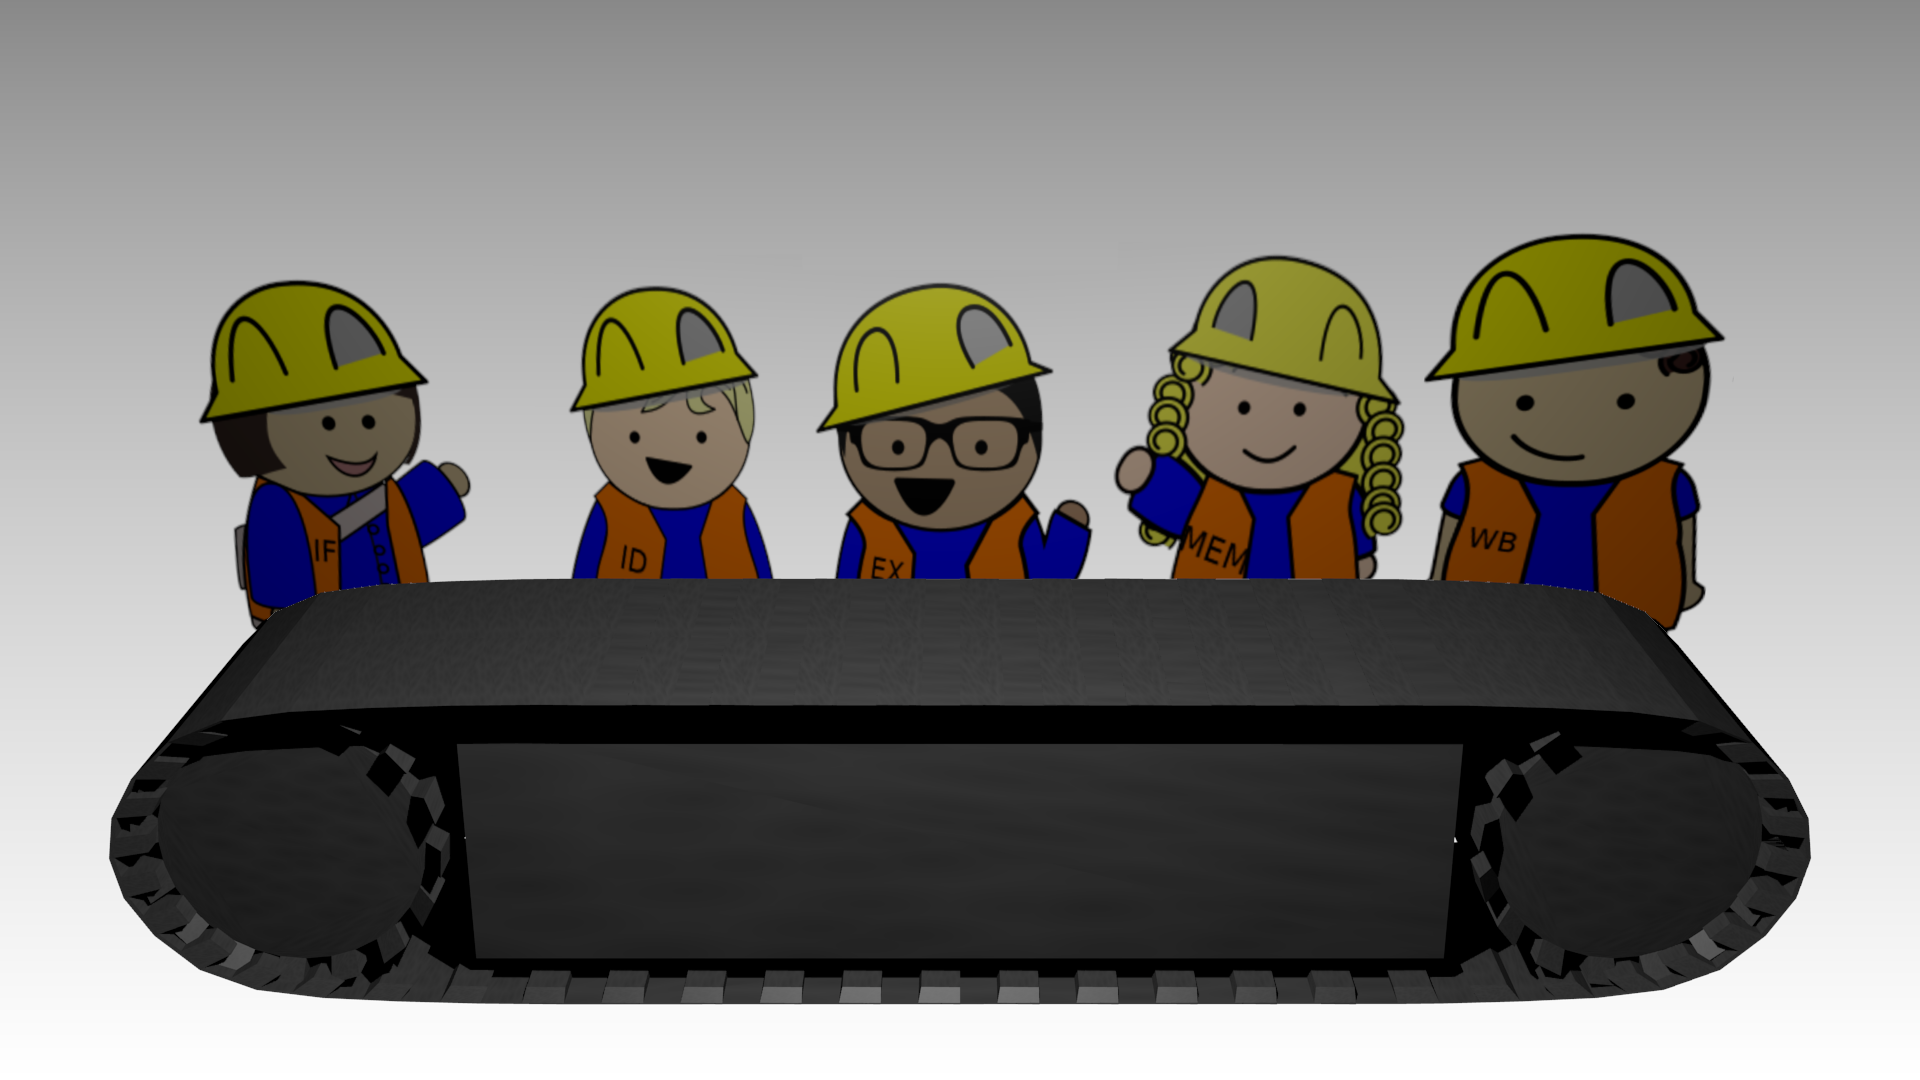
\includegraphics[width=1.0\textwidth]{final.png}}
%FETCH
\put(50,-12){\fontsize{5.5}{4}\selectfont\color{white}nop}

%DECODE
\put(90,-12){\fontsize{5.5}{4}\selectfont\color{white}nop}
\put(90,-17){\fontsize{5.5}{4}\selectfont\color{white}}

%EXECUTE
\put(135,-12){\fontsize{5.5}{4}\selectfont\color{white}add t1, zero, 1}
\put(135,-17){\fontsize{5.5}{4}\selectfont\color{white}t1 = 0 + 1}
\put(135,-22){\fontsize{5.5}{4}\selectfont\color{white}t1 = 1}

%MEMORY
\put(185,-12){\fontsize{5.5}{4}\selectfont\color{white}add t0, zero, 1}
\put(185,-17){\fontsize{5.5}{4}\selectfont\color{white}t0 = 0 + 1}
\put(185,-22){\fontsize{5.5}{4}\selectfont\color{white}t0 = 1}

%WRITEBACK
\put(225,-12){\fontsize{5.5}{4}\selectfont\color{white}}
\put(225,-17){\fontsize{5.5}{4}\selectfont\color{white}}
\put(225,-22){\fontsize{5.5}{4}\selectfont\color{white}}

%REGISTERS
\put(80,-37){\fontsize{5.5}{4}\selectfont\color{white}zero = 0}
\put(80,-42){\fontsize{5.5}{4}\selectfont\color{white}ra = 0}
\put(80,-47){\fontsize{5.5}{4}\selectfont\color{white}sp = 0}
\put(80,-52){\fontsize{5.5}{4}\selectfont\color{white}pc = 12}
\put(80,-57){\fontsize{5.5}{4}\selectfont\color{white}t0 = 0}
\put(80,-62){\fontsize{5.5}{4}\selectfont\color{white}t1 = 0}

\put(110,-37){\fontsize{5.5}{4}\selectfont\color{white}t2 = 0}
\put(110,-42){\fontsize{5.5}{4}\selectfont\color{white}t3 = 0}
\put(110,-47){\fontsize{5.5}{4}\selectfont\color{white}t4 = 0}
\put(110,-52){\fontsize{5.5}{4}\selectfont\color{white}t5 = 0}
\put(110,-57){\fontsize{5.5}{4}\selectfont\color{white}t6 = 0}
\put(110,-62){\fontsize{5.5}{4}\selectfont\color{white}a0 = 0}

\put(140,-37){\fontsize{5.5}{4}\selectfont\color{white}a1 = 0}
\put(140,-42){\fontsize{5.5}{4}\selectfont\color{white}a2 = 0}
\put(140,-47){\fontsize{5.5}{4}\selectfont\color{white}a3 = 0}
\put(140,-52){\fontsize{5.5}{4}\selectfont\color{white}a4 = 0}
\put(140,-57){\fontsize{5.5}{4}\selectfont\color{white}a5 = 0}
\put(140,-62){\fontsize{5.5}{4}\selectfont\color{white}a6 = 0}

\put(170,-37){\fontsize{5.5}{4}\selectfont\color{white}a7 = 0}
\put(170,-42){\fontsize{5.5}{4}\selectfont\color{white}s1 = 0}
\put(170,-47){\fontsize{5.5}{4}\selectfont\color{white}s2 = 0}
\put(170,-52){\fontsize{5.5}{4}\selectfont\color{white}s3 = 0}
\put(170,-57){\fontsize{5.5}{4}\selectfont\color{white}s4 = 0}
\put(170,-62){\fontsize{5.5}{4}\selectfont\color{white}s5 = 0}

\put(200,-37){\fontsize{5.5}{4}\selectfont\color{white}s6 = 0}
\put(200,-42){\fontsize{5.5}{4}\selectfont\color{white}s7 = 0}
\put(200,-47){\fontsize{5.5}{4}\selectfont\color{white}s8 = 0}
\put(200,-52){\fontsize{5.5}{4}\selectfont\color{white}s9 = 0}
\put(200,-57){\fontsize{5.5}{4}\selectfont\color{white}s10 = 0}
\put(200,-62){\fontsize{5.5}{4}\selectfont\color{white}s11 = 0}

\end{picture}
\end{frame}

\begin{frame}
\frametitle{Conditional Branch | Takt 4}
\begin{picture}(0,0)
\put(0,-85){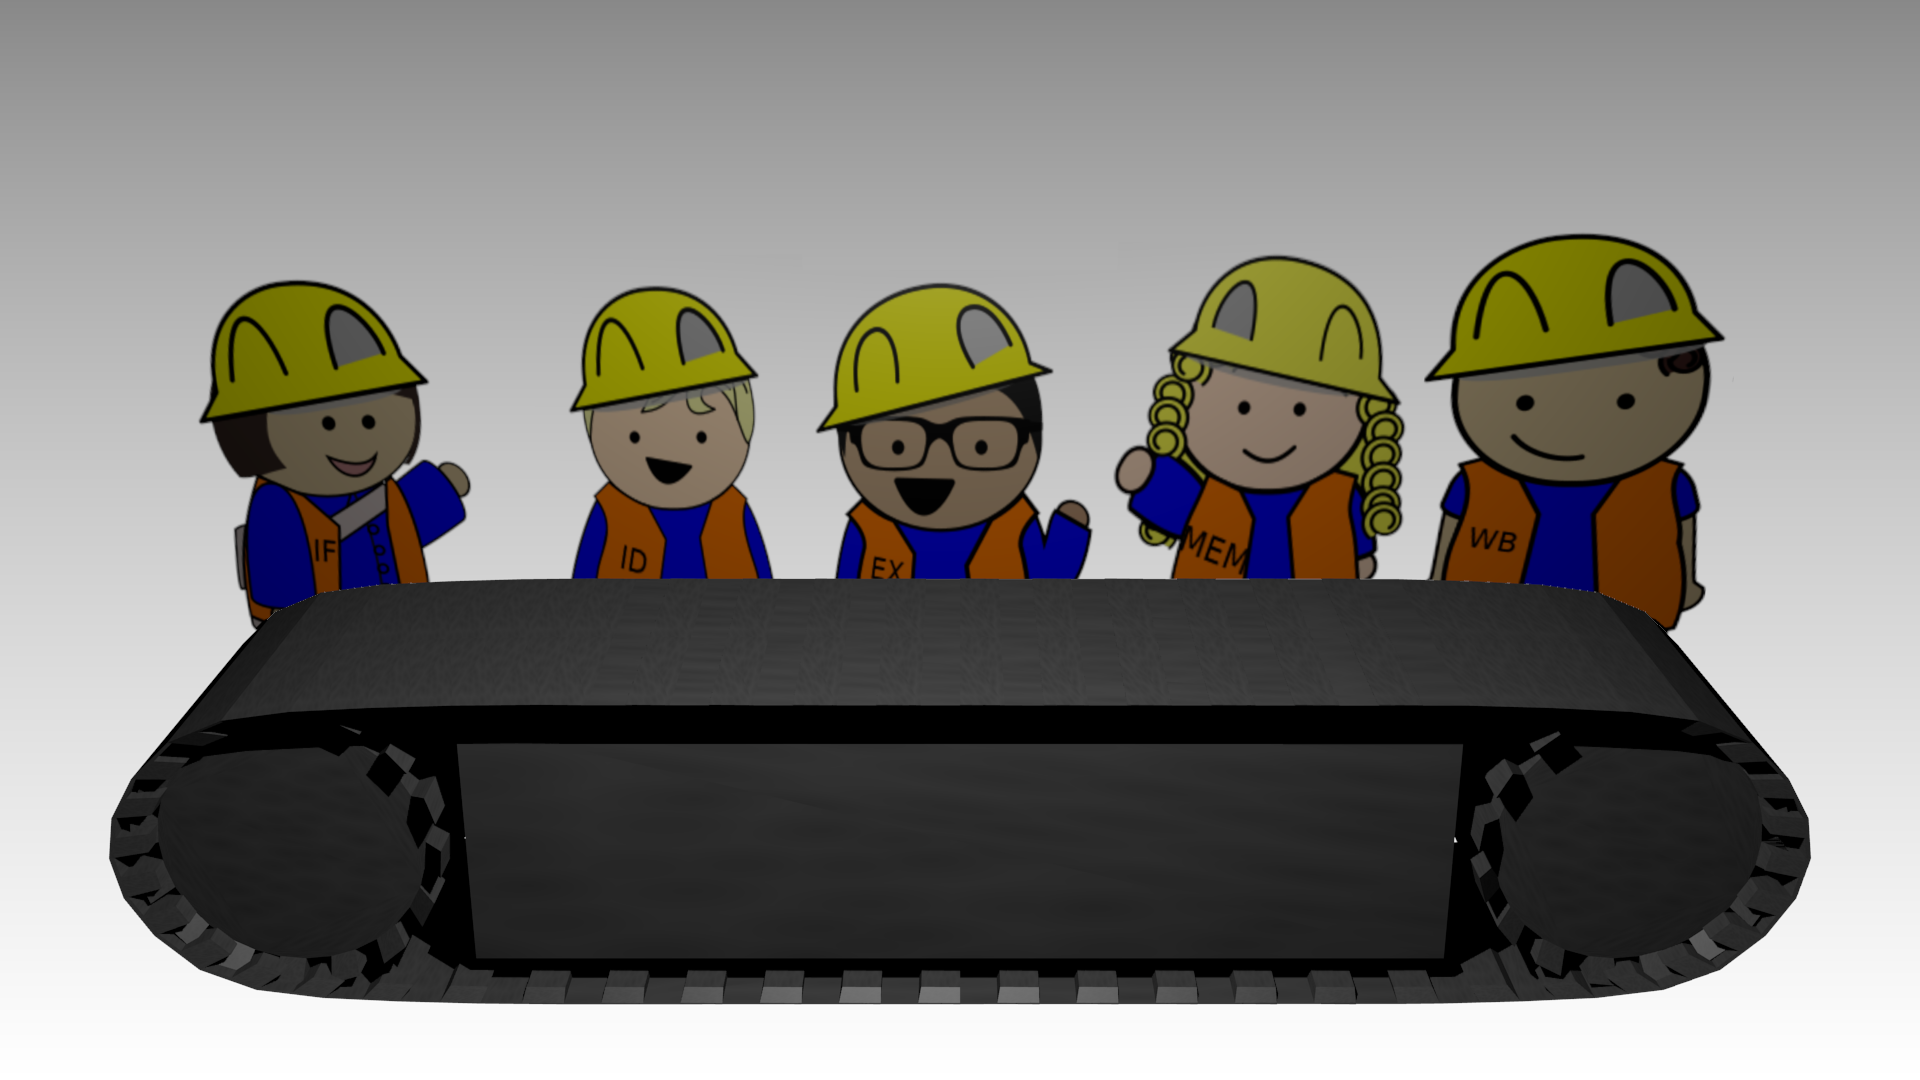
\includegraphics[width=1.0\textwidth]{final.png}}
%FETCH
\put(50,-12){\fontsize{5.5}{4}\selectfont\color{white}beq t0, t1, end}

%DECODE
\put(90,-12){\fontsize{5.5}{4}\selectfont\color{white}nop}
\put(90,-17){\fontsize{5.5}{4}\selectfont\color{white}}

%EXECUTE
\put(135,-12){\fontsize{5.5}{4}\selectfont\color{white}nop}
\put(135,-17){\fontsize{5.5}{4}\selectfont\color{white}}
\put(135,-22){\fontsize{5.5}{4}\selectfont\color{white}}

%MEMORY
\put(185,-12){\fontsize{5.5}{4}\selectfont\color{white}add t1, zero, 1}
\put(185,-17){\fontsize{5.5}{4}\selectfont\color{white}t1 = 0 + 1}
\put(185,-22){\fontsize{5.5}{4}\selectfont\color{white}t1 = 1}

%WRITEBACK
\put(225,-12){\fontsize{5.5}{4}\selectfont\color{white}add t0, zero, 1}
\put(225,-17){\fontsize{5.5}{4}\selectfont\color{white}t0 = 0 + 1}
\put(225,-22){\fontsize{5.5}{4}\selectfont\color{white}t0 = 1}

%REGISTERS
\put(80,-37){\fontsize{5.5}{4}\selectfont\color{white}zero = 0}
\put(80,-42){\fontsize{5.5}{4}\selectfont\color{white}ra = 0}
\put(80,-47){\fontsize{5.5}{4}\selectfont\color{white}sp = 0}
\put(80,-52){\fontsize{5.5}{4}\selectfont\color{white}pc = 16}
\put(80,-57){\fontsize{5.5}{4}\selectfont\color{white}t0 = 1}
\put(80,-62){\fontsize{5.5}{4}\selectfont\color{white}t1 = 0}

\put(110,-37){\fontsize{5.5}{4}\selectfont\color{white}t2 = 0}
\put(110,-42){\fontsize{5.5}{4}\selectfont\color{white}t3 = 0}
\put(110,-47){\fontsize{5.5}{4}\selectfont\color{white}t4 = 0}
\put(110,-52){\fontsize{5.5}{4}\selectfont\color{white}t5 = 0}
\put(110,-57){\fontsize{5.5}{4}\selectfont\color{white}t6 = 0}
\put(110,-62){\fontsize{5.5}{4}\selectfont\color{white}a0 = 0}

\put(140,-37){\fontsize{5.5}{4}\selectfont\color{white}a1 = 0}
\put(140,-42){\fontsize{5.5}{4}\selectfont\color{white}a2 = 0}
\put(140,-47){\fontsize{5.5}{4}\selectfont\color{white}a3 = 0}
\put(140,-52){\fontsize{5.5}{4}\selectfont\color{white}a4 = 0}
\put(140,-57){\fontsize{5.5}{4}\selectfont\color{white}a5 = 0}
\put(140,-62){\fontsize{5.5}{4}\selectfont\color{white}a6 = 0}

\put(170,-37){\fontsize{5.5}{4}\selectfont\color{white}a7 = 0}
\put(170,-42){\fontsize{5.5}{4}\selectfont\color{white}s1 = 0}
\put(170,-47){\fontsize{5.5}{4}\selectfont\color{white}s2 = 0}
\put(170,-52){\fontsize{5.5}{4}\selectfont\color{white}s3 = 0}
\put(170,-57){\fontsize{5.5}{4}\selectfont\color{white}s4 = 0}
\put(170,-62){\fontsize{5.5}{4}\selectfont\color{white}s5 = 0}

\put(200,-37){\fontsize{5.5}{4}\selectfont\color{white}s6 = 0}
\put(200,-42){\fontsize{5.5}{4}\selectfont\color{white}s7 = 0}
\put(200,-47){\fontsize{5.5}{4}\selectfont\color{white}s8 = 0}
\put(200,-52){\fontsize{5.5}{4}\selectfont\color{white}s9 = 0}
\put(200,-57){\fontsize{5.5}{4}\selectfont\color{white}s10 = 0}
\put(200,-62){\fontsize{5.5}{4}\selectfont\color{white}s11 = 0}

\end{picture}
\end{frame}


\begin{frame}
\frametitle{Conditional Branch | Takt 5}
\begin{picture}(0,0)
\put(0,-85){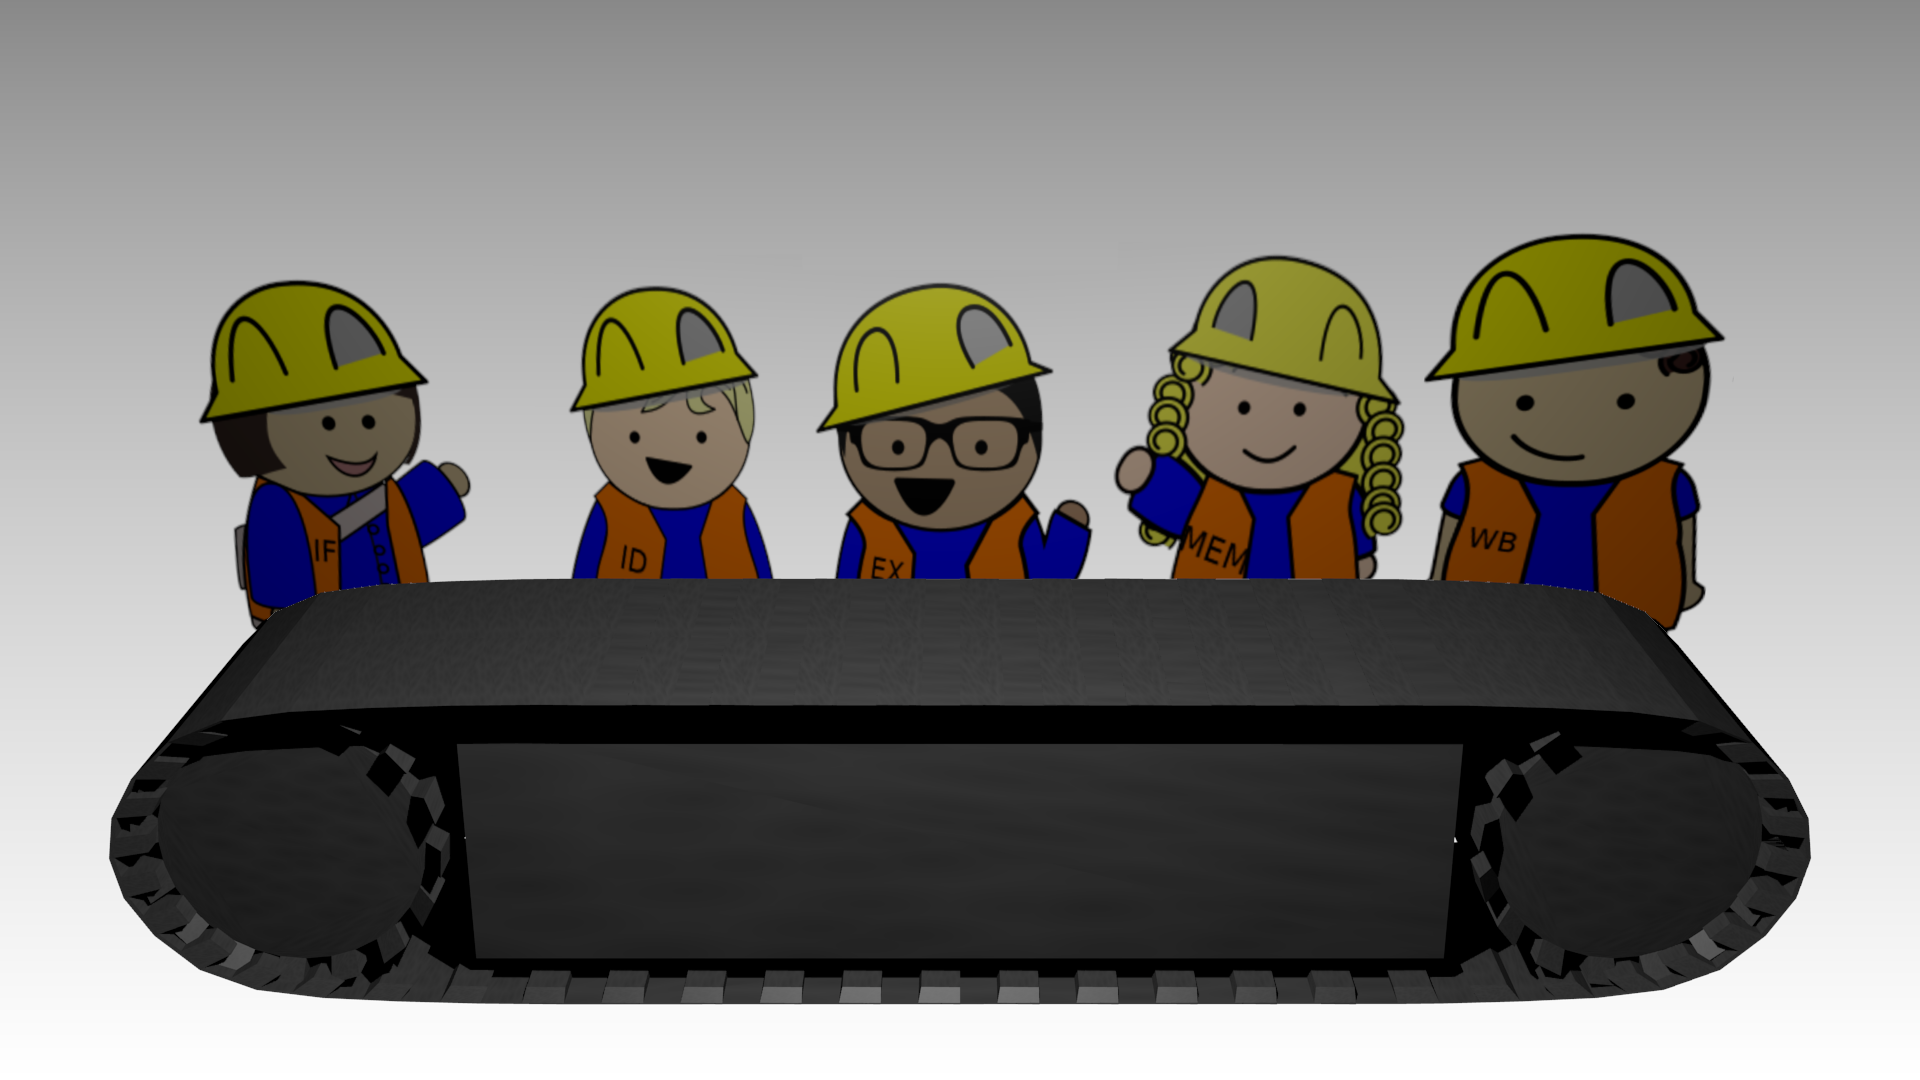
\includegraphics[width=1.0\textwidth]{final.png}}
%FETCH
\put(50,-12){\fontsize{5.5}{4}\selectfont\color{white}add t2, zero, 3}

%DECODE
\put(90,-12){\fontsize{5.5}{4}\selectfont\color{white}beq t0, t1, end}
\put(85,-17){\fontsize{4}{3}\selectfont\color{white}pc=(1==1)?16+20:16+4}

%EXECUTE
\put(135,-12){\fontsize{5.5}{4}\selectfont\color{white}nop}
\put(135,-17){\fontsize{5.5}{4}\selectfont\color{white}}
\put(135,-22){\fontsize{5.5}{4}\selectfont\color{white}}

%MEMORY
\put(185,-12){\fontsize{5.5}{4}\selectfont\color{white}nop}
\put(185,-17){\fontsize{5.5}{4}\selectfont\color{white}}
\put(185,-22){\fontsize{5.5}{4}\selectfont\color{white}}

%WRITEBACK
\put(225,-12){\fontsize{5.5}{4}\selectfont\color{white}add t1, zero, 1}
\put(225,-17){\fontsize{5.5}{4}\selectfont\color{white}t1 = 0 + 1}
\put(225,-22){\fontsize{5.5}{4}\selectfont\color{white}t1 = 1}

%REGISTERS
\put(80,-37){\fontsize{5.5}{4}\selectfont\color{white}zero = 0}
\put(80,-42){\fontsize{5.5}{4}\selectfont\color{white}ra = 0}
\put(80,-47){\fontsize{5.5}{4}\selectfont\color{white}sp = 0}
\put(80,-52){\fontsize{5.5}{4}\selectfont\color{white}pc = 20}
\put(80,-57){\fontsize{5.5}{4}\selectfont\color{white}t0 = 1}
\put(80,-62){\fontsize{5.5}{4}\selectfont\color{white}t1 = 1}

\put(110,-37){\fontsize{5.5}{4}\selectfont\color{white}t2 = 0}
\put(110,-42){\fontsize{5.5}{4}\selectfont\color{white}t3 = 0}
\put(110,-47){\fontsize{5.5}{4}\selectfont\color{white}t4 = 0}
\put(110,-52){\fontsize{5.5}{4}\selectfont\color{white}t5 = 0}
\put(110,-57){\fontsize{5.5}{4}\selectfont\color{white}t6 = 0}
\put(110,-62){\fontsize{5.5}{4}\selectfont\color{white}a0 = 0}

\put(140,-37){\fontsize{5.5}{4}\selectfont\color{white}a1 = 0}
\put(140,-42){\fontsize{5.5}{4}\selectfont\color{white}a2 = 0}
\put(140,-47){\fontsize{5.5}{4}\selectfont\color{white}a3 = 0}
\put(140,-52){\fontsize{5.5}{4}\selectfont\color{white}a4 = 0}
\put(140,-57){\fontsize{5.5}{4}\selectfont\color{white}a5 = 0}
\put(140,-62){\fontsize{5.5}{4}\selectfont\color{white}a6 = 0}

\put(170,-37){\fontsize{5.5}{4}\selectfont\color{white}a7 = 0}
\put(170,-42){\fontsize{5.5}{4}\selectfont\color{white}s1 = 0}
\put(170,-47){\fontsize{5.5}{4}\selectfont\color{white}s2 = 0}
\put(170,-52){\fontsize{5.5}{4}\selectfont\color{white}s3 = 0}
\put(170,-57){\fontsize{5.5}{4}\selectfont\color{white}s4 = 0}
\put(170,-62){\fontsize{5.5}{4}\selectfont\color{white}s5 = 0}

\put(200,-37){\fontsize{5.5}{4}\selectfont\color{white}s6 = 0}
\put(200,-42){\fontsize{5.5}{4}\selectfont\color{white}s7 = 0}
\put(200,-47){\fontsize{5.5}{4}\selectfont\color{white}s8 = 0}
\put(200,-52){\fontsize{5.5}{4}\selectfont\color{white}s9 = 0}
\put(200,-57){\fontsize{5.5}{4}\selectfont\color{white}s10 = 0}
\put(200,-62){\fontsize{5.5}{4}\selectfont\color{white}s11 = 0}

\end{picture}
\end{frame}

\begin{frame}
\frametitle{Conditional Branch | Takt 6}
\begin{picture}(0,0)
\put(0,-85){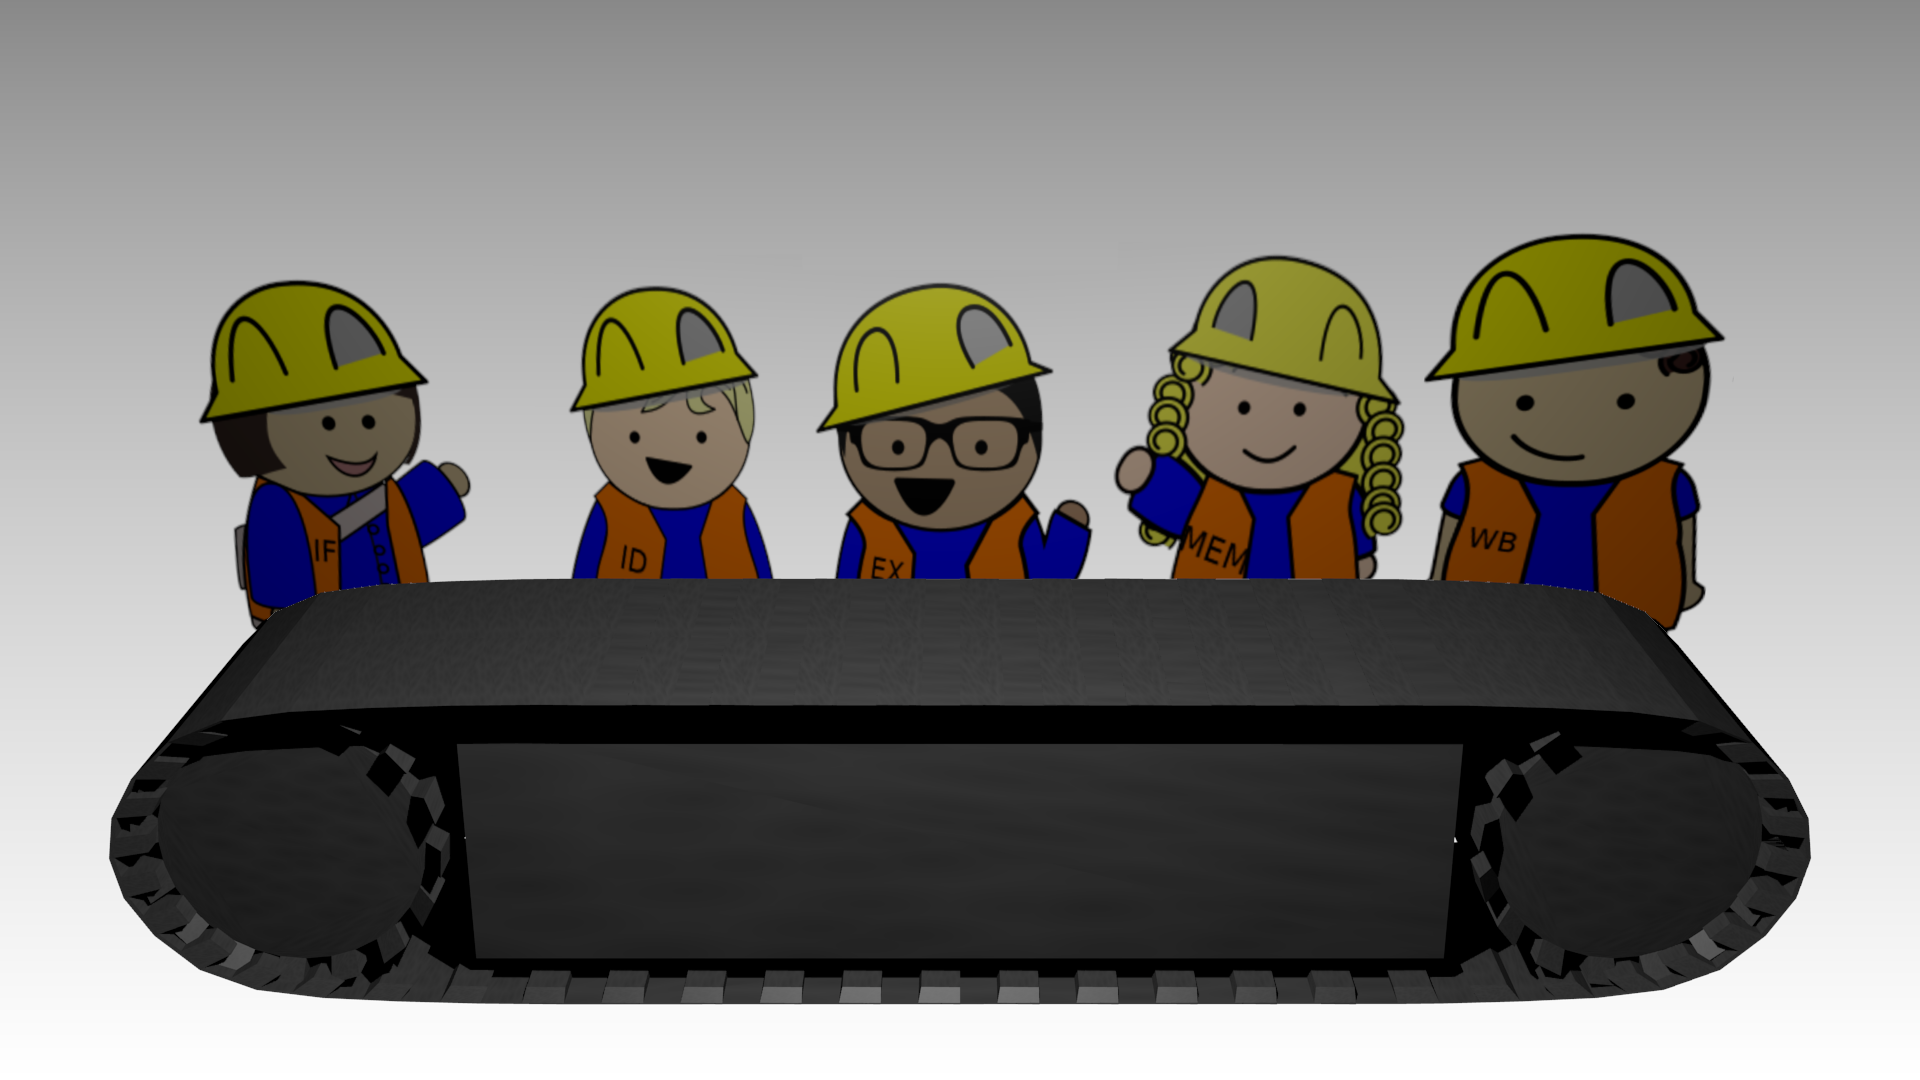
\includegraphics[width=1.0\textwidth]{final.png}}
%FETCH
\put(50,-12){\fontsize{5.5}{4}\selectfont\color{white}add t3, zero, 4}

%DECODE
\put(90,-12){\fontsize{5.5}{4}\selectfont\color{white}add t2, zero, 3}
\put(90,-17){\fontsize{5.5}{4}\selectfont\color{white}t2 = 0 + 3}

%EXECUTE
\put(135,-12){\fontsize{5.5}{4}\selectfont\color{white}beq t0, t1, end}
\put(130,-17){\fontsize{4}{3}\selectfont\color{white}pc=(1==1)?16+20:16+4}
\put(130,-22){\fontsize{4}{3}\selectfont\color{white}pc=(TRUE)?36:20}

%MEMORY
\put(185,-12){\fontsize{5.5}{4}\selectfont\color{white}nop}
\put(185,-17){\fontsize{5.5}{4}\selectfont\color{white}}
\put(185,-22){\fontsize{5.5}{4}\selectfont\color{white}}

%WRITEBACK
\put(225,-12){\fontsize{5.5}{4}\selectfont\color{white}nop}
\put(225,-17){\fontsize{5.5}{4}\selectfont\color{white}}
\put(225,-22){\fontsize{5.5}{4}\selectfont\color{white}}

%REGISTERS
\put(80,-37){\fontsize{5.5}{4}\selectfont\color{white}zero = 0}
\put(80,-42){\fontsize{5.5}{4}\selectfont\color{white}ra = 0}
\put(80,-47){\fontsize{5.5}{4}\selectfont\color{white}sp = 0}
\put(80,-52){\fontsize{5.5}{4}\selectfont\color{white}pc = 24}
\put(80,-57){\fontsize{5.5}{4}\selectfont\color{white}t0 = 1}
\put(80,-62){\fontsize{5.5}{4}\selectfont\color{white}t1 = 1}

\put(110,-37){\fontsize{5.5}{4}\selectfont\color{white}t2 = 0}
\put(110,-42){\fontsize{5.5}{4}\selectfont\color{white}t3 = 0}
\put(110,-47){\fontsize{5.5}{4}\selectfont\color{white}t4 = 0}
\put(110,-52){\fontsize{5.5}{4}\selectfont\color{white}t5 = 0}
\put(110,-57){\fontsize{5.5}{4}\selectfont\color{white}t6 = 0}
\put(110,-62){\fontsize{5.5}{4}\selectfont\color{white}a0 = 0}

\put(140,-37){\fontsize{5.5}{4}\selectfont\color{white}a1 = 0}
\put(140,-42){\fontsize{5.5}{4}\selectfont\color{white}a2 = 0}
\put(140,-47){\fontsize{5.5}{4}\selectfont\color{white}a3 = 0}
\put(140,-52){\fontsize{5.5}{4}\selectfont\color{white}a4 = 0}
\put(140,-57){\fontsize{5.5}{4}\selectfont\color{white}a5 = 0}
\put(140,-62){\fontsize{5.5}{4}\selectfont\color{white}a6 = 0}

\put(170,-37){\fontsize{5.5}{4}\selectfont\color{white}a7 = 0}
\put(170,-42){\fontsize{5.5}{4}\selectfont\color{white}s1 = 0}
\put(170,-47){\fontsize{5.5}{4}\selectfont\color{white}s2 = 0}
\put(170,-52){\fontsize{5.5}{4}\selectfont\color{white}s3 = 0}
\put(170,-57){\fontsize{5.5}{4}\selectfont\color{white}s4 = 0}
\put(170,-62){\fontsize{5.5}{4}\selectfont\color{white}s5 = 0}

\put(200,-37){\fontsize{5.5}{4}\selectfont\color{white}s6 = 0}
\put(200,-42){\fontsize{5.5}{4}\selectfont\color{white}s7 = 0}
\put(200,-47){\fontsize{5.5}{4}\selectfont\color{white}s8 = 0}
\put(200,-52){\fontsize{5.5}{4}\selectfont\color{white}s9 = 0}
\put(200,-57){\fontsize{5.5}{4}\selectfont\color{white}s10 = 0}
\put(200,-62){\fontsize{5.5}{4}\selectfont\color{white}s11 = 0}

\end{picture}
\end{frame}

\begin{frame}
\frametitle{Conditional Branch | Takt 7}
\begin{picture}(0,0)
\put(0,-85){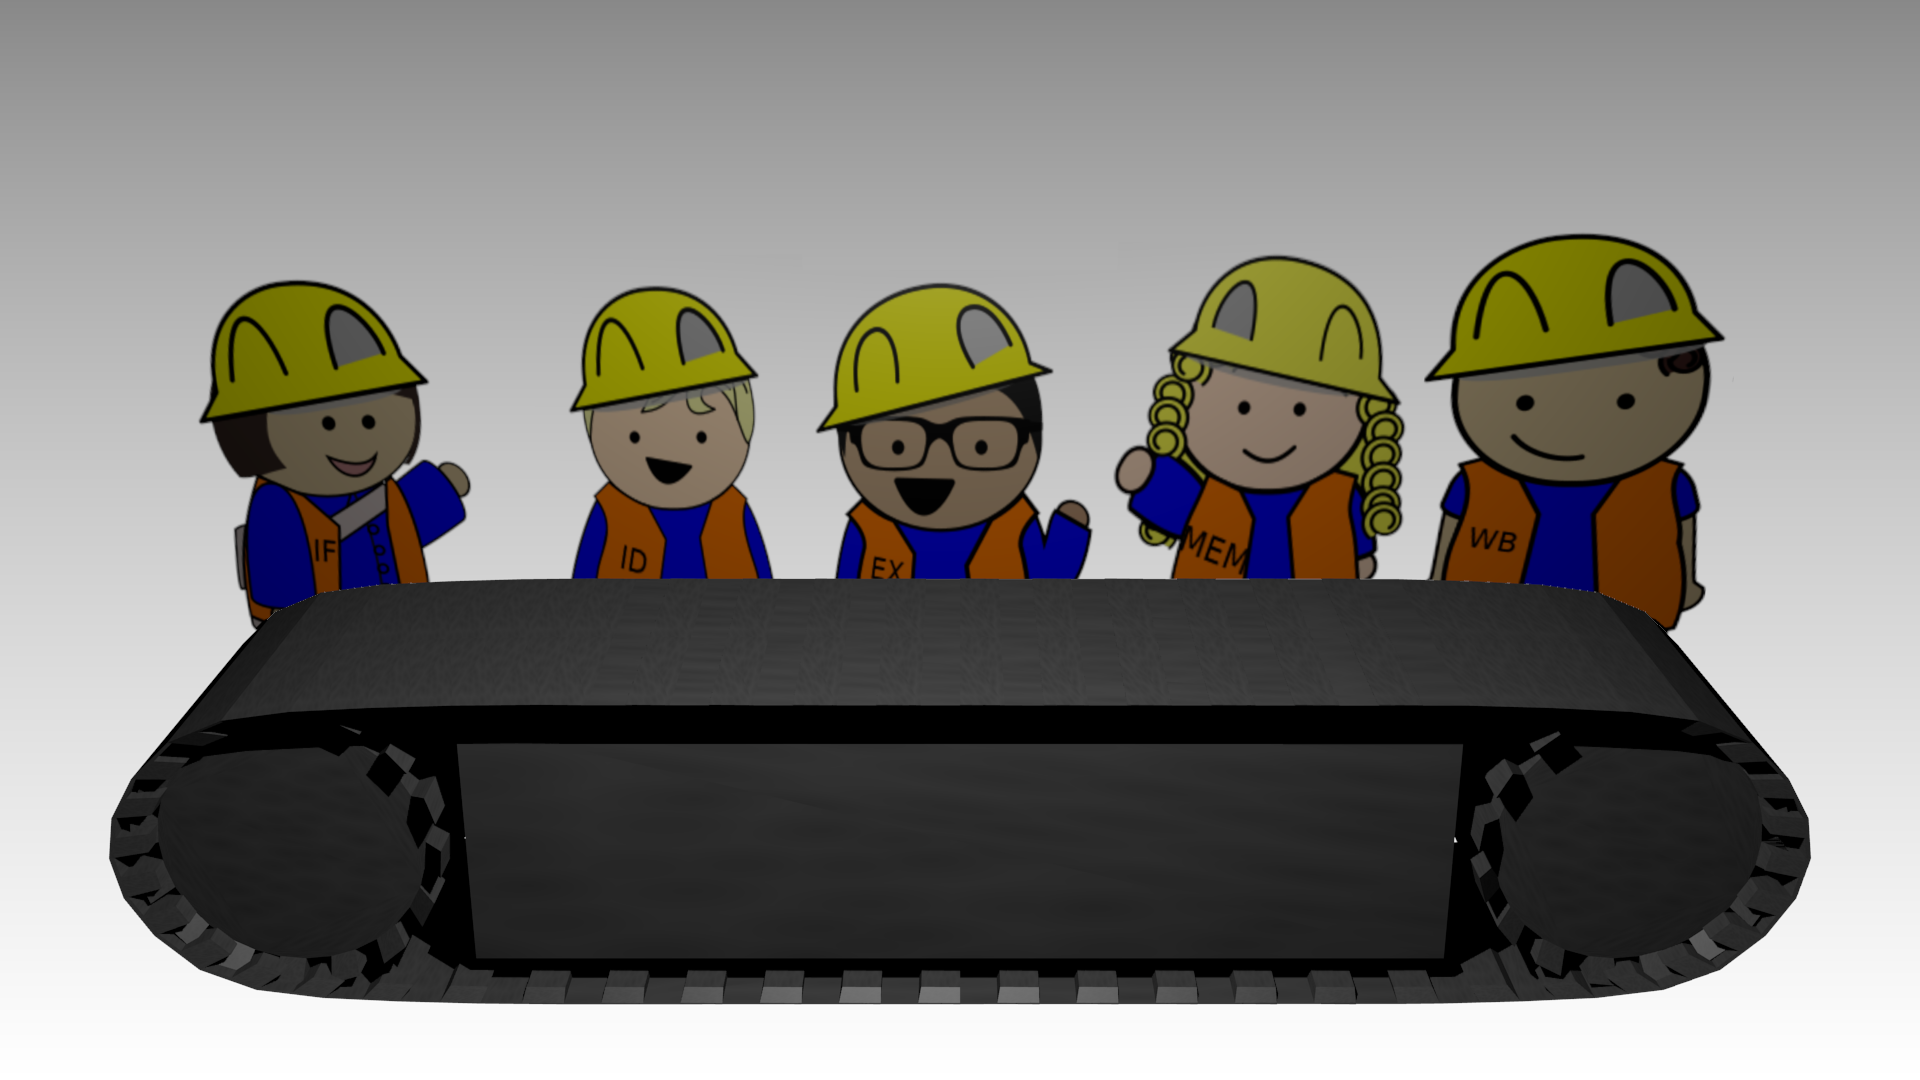
\includegraphics[width=1.0\textwidth]{final.png}}
%FETCH
\put(50,-12){\fontsize{5.5}{4}\selectfont\color{white}add t4, zero, 5}

%DECODE
\put(90,-12){\fontsize{5.5}{4}\selectfont\color{white}add t3, zero, 4}
\put(90,-17){\fontsize{5.5}{4}\selectfont\color{white}t3 = 0 + 4}

%EXECUTE
\put(135,-12){\fontsize{5.5}{4}\selectfont\color{white}add t2, zero, 3}
\put(135,-17){\fontsize{5.5}{4}\selectfont\color{white}t2 = 0 + 3}
\put(135,-22){\fontsize{5.5}{4}\selectfont\color{white}t2 = 3}

%MEMORY
\put(180,-10){\fontsize{5.5}{4}\selectfont\color{white}beq t0, t1, end}
\put(180,-15){\fontsize{4}{3}\selectfont\color{white}pc=(1 == 1)?16+20:16+4}
\put(180,-20){\fontsize{4}{3}\selectfont\color{white}pc=(TRUE)?36:20}
\put(180,-25){\fontsize{4}{3}\selectfont\color{white}pc = 36}

%WRITEBACK
\put(225,-12){\fontsize{5.5}{4}\selectfont\color{white}nop}
\put(225,-17){\fontsize{5.5}{4}\selectfont\color{white}}
\put(225,-22){\fontsize{5.5}{4}\selectfont\color{white}}

%REGISTERS
\put(80,-37){\fontsize{5.5}{4}\selectfont\color{white}zero = 0}
\put(80,-42){\fontsize{5.5}{4}\selectfont\color{white}ra = 0}
\put(80,-47){\fontsize{5.5}{4}\selectfont\color{white}sp = 0}
\put(80,-52){\fontsize{5.5}{4}\selectfont\color{white}pc = 28}
\put(80,-57){\fontsize{5.5}{4}\selectfont\color{white}t0 = 1}
\put(80,-62){\fontsize{5.5}{4}\selectfont\color{white}t1 = 1}

\put(110,-37){\fontsize{5.5}{4}\selectfont\color{white}t2 = 0}
\put(110,-42){\fontsize{5.5}{4}\selectfont\color{white}t3 = 0}
\put(110,-47){\fontsize{5.5}{4}\selectfont\color{white}t4 = 0}
\put(110,-52){\fontsize{5.5}{4}\selectfont\color{white}t5 = 0}
\put(110,-57){\fontsize{5.5}{4}\selectfont\color{white}t6 = 0}
\put(110,-62){\fontsize{5.5}{4}\selectfont\color{white}a0 = 0}

\put(140,-37){\fontsize{5.5}{4}\selectfont\color{white}a1 = 0}
\put(140,-42){\fontsize{5.5}{4}\selectfont\color{white}a2 = 0}
\put(140,-47){\fontsize{5.5}{4}\selectfont\color{white}a3 = 0}
\put(140,-52){\fontsize{5.5}{4}\selectfont\color{white}a4 = 0}
\put(140,-57){\fontsize{5.5}{4}\selectfont\color{white}a5 = 0}
\put(140,-62){\fontsize{5.5}{4}\selectfont\color{white}a6 = 0}

\put(170,-37){\fontsize{5.5}{4}\selectfont\color{white}a7 = 0}
\put(170,-42){\fontsize{5.5}{4}\selectfont\color{white}s1 = 0}
\put(170,-47){\fontsize{5.5}{4}\selectfont\color{white}s2 = 0}
\put(170,-52){\fontsize{5.5}{4}\selectfont\color{white}s3 = 0}
\put(170,-57){\fontsize{5.5}{4}\selectfont\color{white}s4 = 0}
\put(170,-62){\fontsize{5.5}{4}\selectfont\color{white}s5 = 0}

\put(200,-37){\fontsize{5.5}{4}\selectfont\color{white}s6 = 0}
\put(200,-42){\fontsize{5.5}{4}\selectfont\color{white}s7 = 0}
\put(200,-47){\fontsize{5.5}{4}\selectfont\color{white}s8 = 0}
\put(200,-52){\fontsize{5.5}{4}\selectfont\color{white}s9 = 0}
\put(200,-57){\fontsize{5.5}{4}\selectfont\color{white}s10 = 0}
\put(200,-62){\fontsize{5.5}{4}\selectfont\color{white}s11 = 0}

\end{picture}
\end{frame}

\begin{frame}
\frametitle{Conditional Branch | Takt 8}
\begin{picture}(0,0)
\put(0,-85){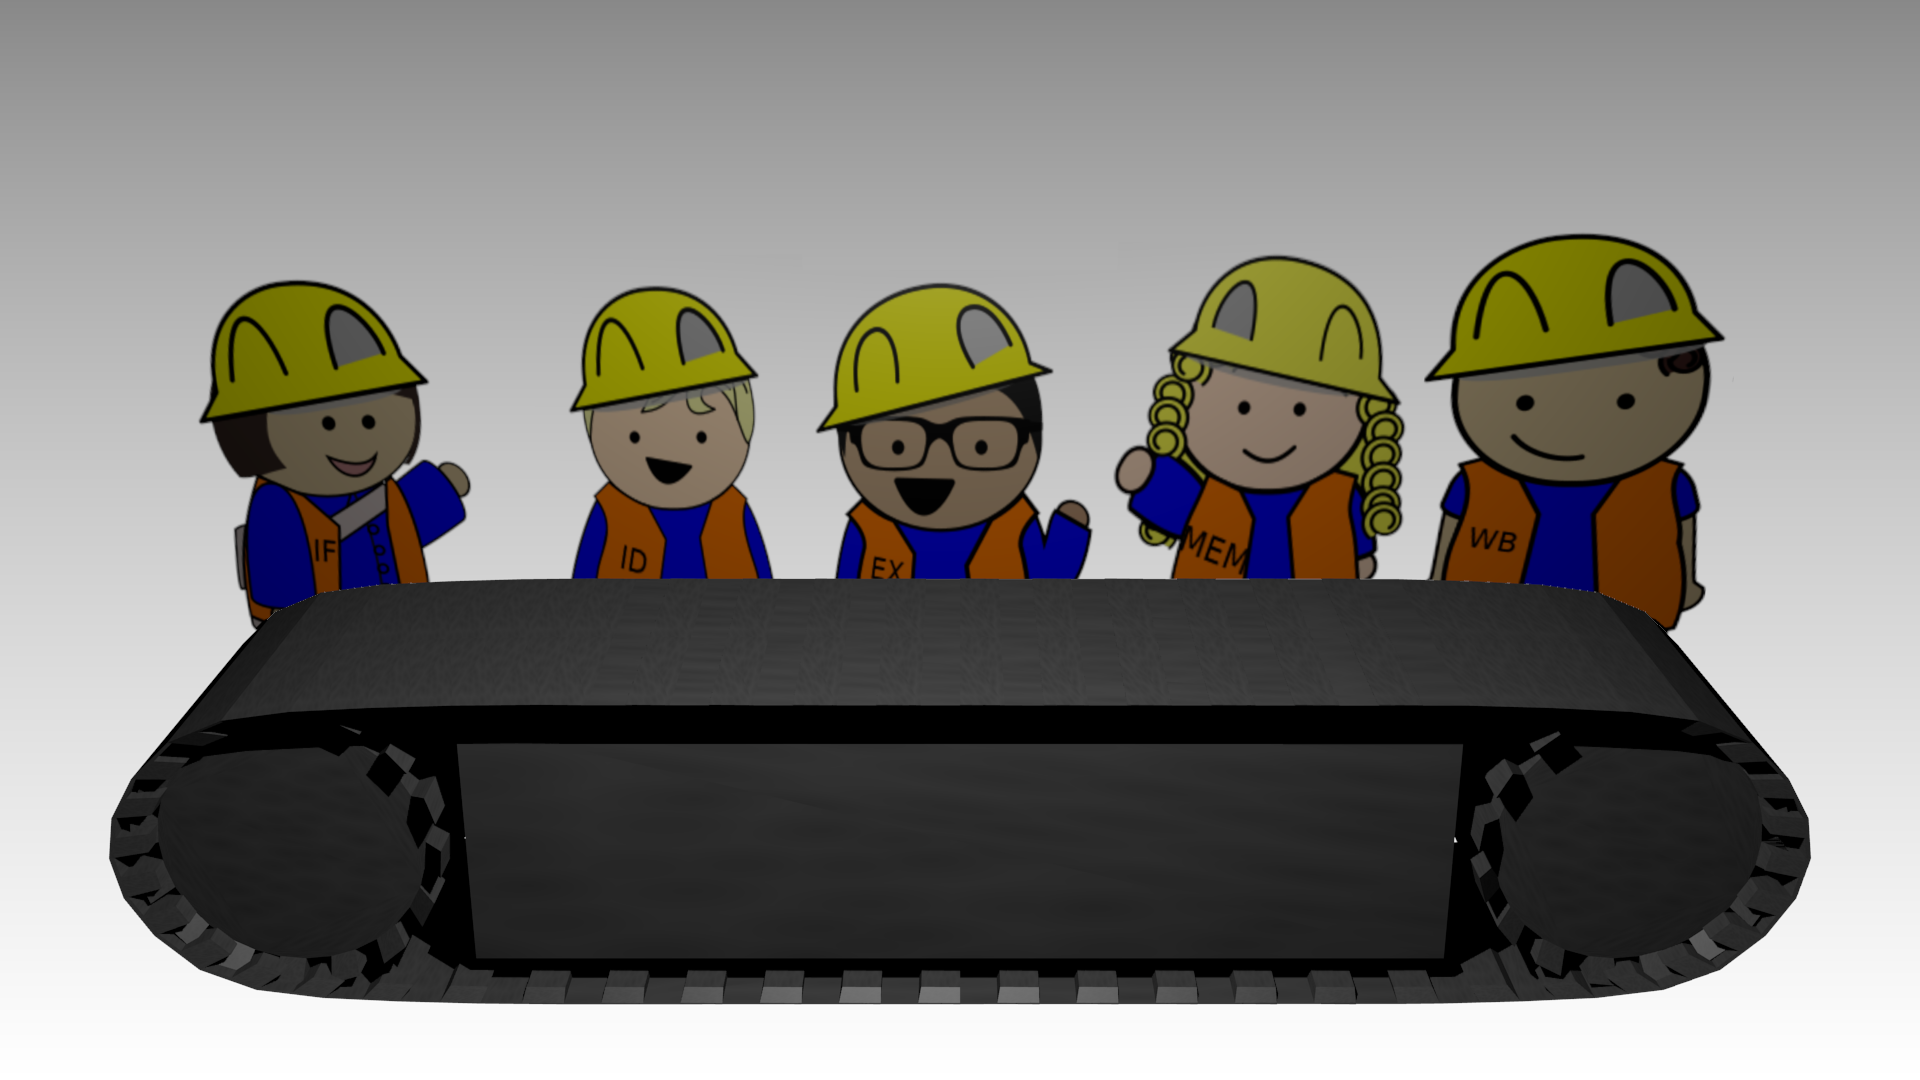
\includegraphics[width=1.0\textwidth]{final.png}}
%FETCH
\put(50,-12){\fontsize{5.5}{4}\selectfont\color{white}mul t0, t1, t2}

%DECODE
\put(90,-12){\fontsize{5.5}{4}\selectfont\color{white}add t4, zero, 5}
\put(90,-17){\fontsize{5.5}{4}\selectfont\color{white}t4 = 0 + 5}

%EXECUTE
\put(135,-12){\fontsize{5.5}{4}\selectfont\color{white}add t3, zero, 4}
\put(135,-17){\fontsize{5.5}{4}\selectfont\color{white}t3 = 0 + 4}
\put(135,-22){\fontsize{5.5}{4}\selectfont\color{white}t3 = 4}

%MEMORY
\put(185,-12){\fontsize{5.5}{4}\selectfont\color{white}add t2, zero, 3}
\put(185,-17){\fontsize{5.5}{4}\selectfont\color{white}t2 = 0 + 3}
\put(185,-22){\fontsize{5.5}{4}\selectfont\color{white}t2 = 3}

%WRITEBACK
\put(220,-10){\fontsize{5.5}{4}\selectfont\color{white}beq t0, t1, end}
\put(220,-15){\fontsize{4}{3}\selectfont\color{white}pc=(1==1)?16+20:16+4}
\put(220,-20){\fontsize{4}{3}\selectfont\color{white}pc=(TRUE)?36:20}
\put(220,-25){\fontsize{4}{3}\selectfont\color{white}pc = 36}

%REGISTERS
\put(80,-37){\fontsize{5.5}{4}\selectfont\color{white}zero = 0}
\put(80,-42){\fontsize{5.5}{4}\selectfont\color{white}ra = 0}
\put(80,-47){\fontsize{5.5}{4}\selectfont\color{white}sp = 0}
\put(80,-52){\fontsize{5.5}{4}\selectfont\color{white}pc = 36}
\put(80,-57){\fontsize{5.5}{4}\selectfont\color{white}t0 = 1}
\put(80,-62){\fontsize{5.5}{4}\selectfont\color{white}t1 = 1}

\put(110,-37){\fontsize{5.5}{4}\selectfont\color{white}t2 = 0}
\put(110,-42){\fontsize{5.5}{4}\selectfont\color{white}t3 = 0}
\put(110,-47){\fontsize{5.5}{4}\selectfont\color{white}t4 = 0}
\put(110,-52){\fontsize{5.5}{4}\selectfont\color{white}t5 = 0}
\put(110,-57){\fontsize{5.5}{4}\selectfont\color{white}t6 = 0}
\put(110,-62){\fontsize{5.5}{4}\selectfont\color{white}a0 = 0}

\put(140,-37){\fontsize{5.5}{4}\selectfont\color{white}a1 = 0}
\put(140,-42){\fontsize{5.5}{4}\selectfont\color{white}a2 = 0}
\put(140,-47){\fontsize{5.5}{4}\selectfont\color{white}a3 = 0}
\put(140,-52){\fontsize{5.5}{4}\selectfont\color{white}a4 = 0}
\put(140,-57){\fontsize{5.5}{4}\selectfont\color{white}a5 = 0}
\put(140,-62){\fontsize{5.5}{4}\selectfont\color{white}a6 = 0}

\put(170,-37){\fontsize{5.5}{4}\selectfont\color{white}a7 = 0}
\put(170,-42){\fontsize{5.5}{4}\selectfont\color{white}s1 = 0}
\put(170,-47){\fontsize{5.5}{4}\selectfont\color{white}s2 = 0}
\put(170,-52){\fontsize{5.5}{4}\selectfont\color{white}s3 = 0}
\put(170,-57){\fontsize{5.5}{4}\selectfont\color{white}s4 = 0}
\put(170,-62){\fontsize{5.5}{4}\selectfont\color{white}s5 = 0}

\put(200,-37){\fontsize{5.5}{4}\selectfont\color{white}s6 = 0}
\put(200,-42){\fontsize{5.5}{4}\selectfont\color{white}s7 = 0}
\put(200,-47){\fontsize{5.5}{4}\selectfont\color{white}s8 = 0}
\put(200,-52){\fontsize{5.5}{4}\selectfont\color{white}s9 = 0}
\put(200,-57){\fontsize{5.5}{4}\selectfont\color{white}s10 = 0}
\put(200,-62){\fontsize{5.5}{4}\selectfont\color{white}s11 = 0}

\end{picture}
\end{frame}


\begin{frame}
\frametitle{Conditional Branch | Takt 9}
\begin{picture}(0,0)
\put(0,-85){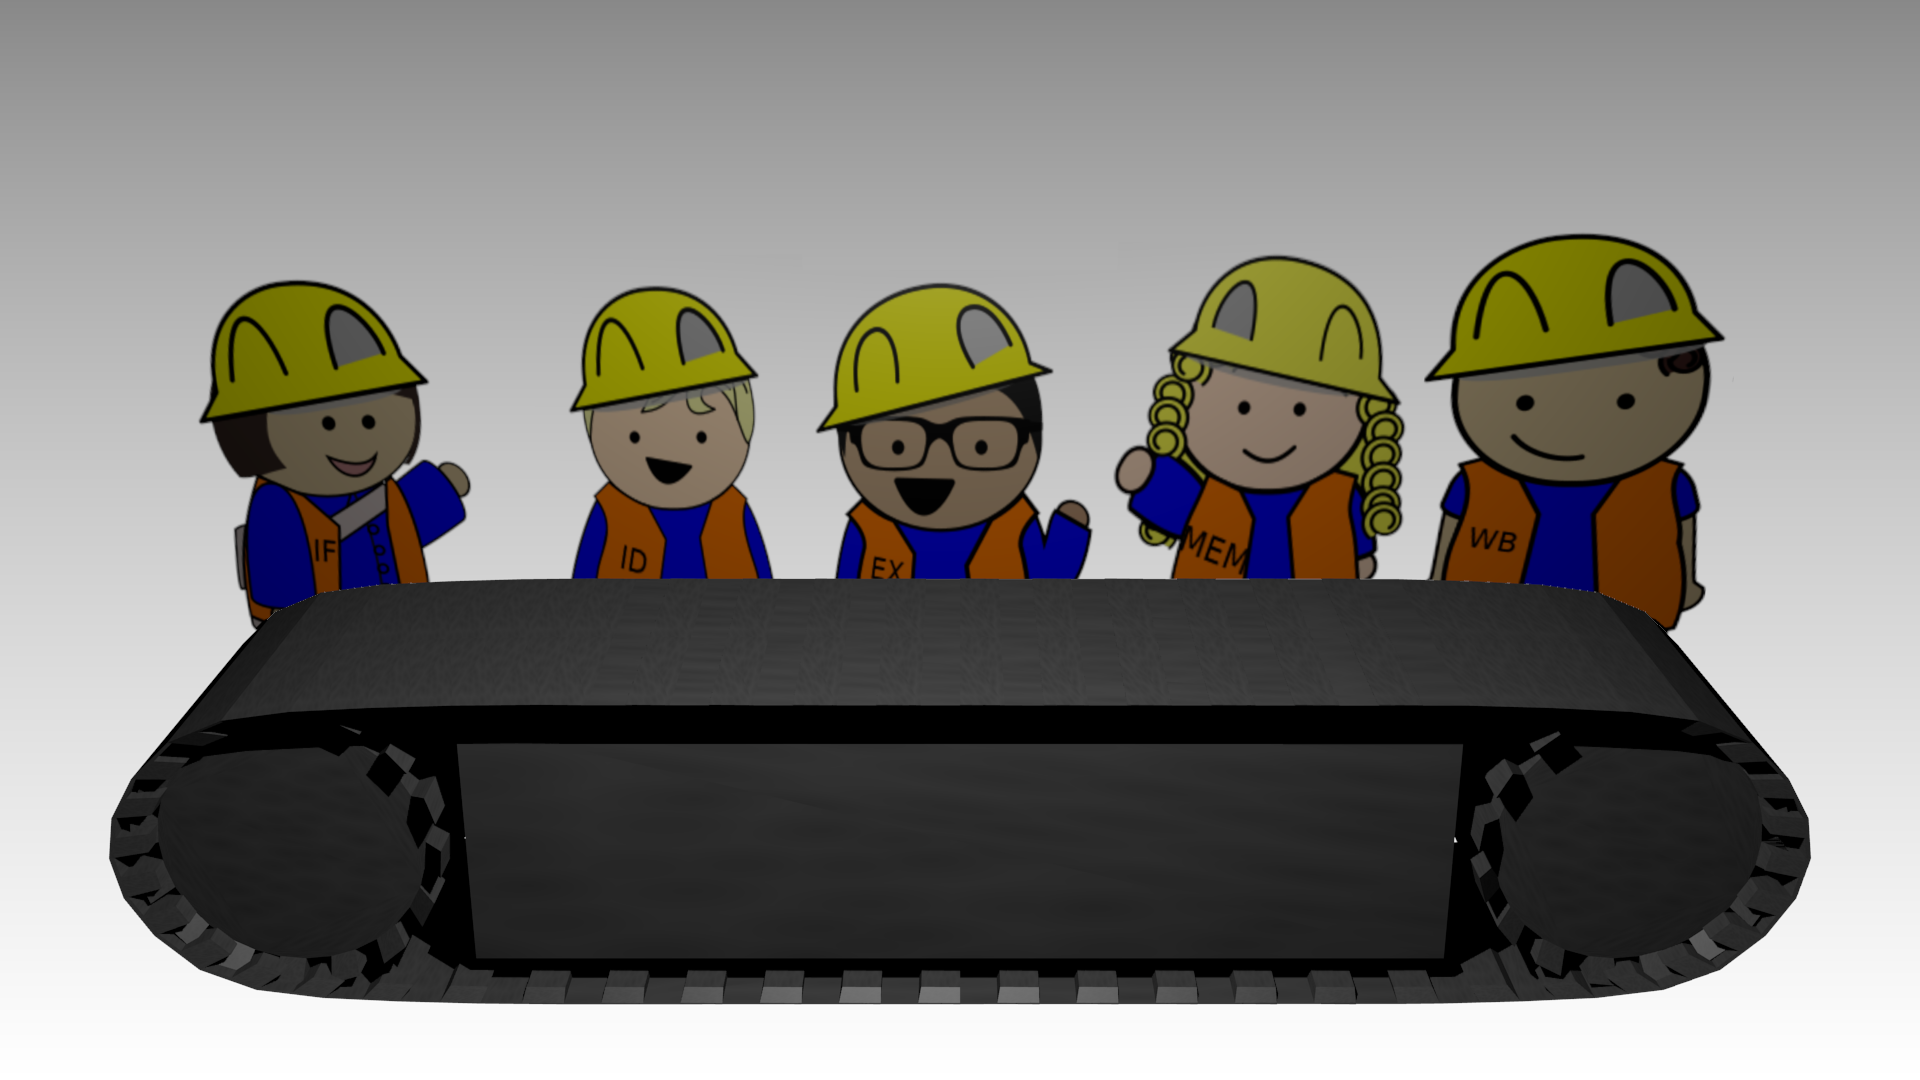
\includegraphics[width=1.0\textwidth]{final.png}}
%FETCH
\put(50,-12){\fontsize{5.5}{4}\selectfont\color{white}}

%DECODE
\put(90,-12){\fontsize{5.5}{4}\selectfont\color{white}mul t0, t1, t2}
\put(90,-17){\fontsize{5.5}{4}\selectfont\color{white}t0 = 1 * 3}

%EXECUTE
\put(135,-12){\fontsize{5.5}{4}\selectfont\color{white}add t4, zero, 5}
\put(135,-17){\fontsize{5.5}{4}\selectfont\color{white}t4 = 0 + 5}
\put(135,-22){\fontsize{5.5}{4}\selectfont\color{white}t4 = 5}

%MEMORY
\put(185,-12){\fontsize{5.5}{4}\selectfont\color{white}add t3, zero, 4}
\put(185,-17){\fontsize{5.5}{4}\selectfont\color{white}t3 = 0 + 4}
\put(185,-22){\fontsize{5.5}{4}\selectfont\color{white}t3 = 4}

%WRITEBACK
\put(225,-12){\fontsize{5.5}{4}\selectfont\color{white}add t2, zero, 3}
\put(225,-17){\fontsize{5.5}{4}\selectfont\color{white}t2 = 0 + 3}
\put(225,-22){\fontsize{5.5}{4}\selectfont\color{white}t2 = 3}

%REGISTERS
\put(80,-37){\fontsize{5.5}{4}\selectfont\color{white}zero = 0}
\put(80,-42){\fontsize{5.5}{4}\selectfont\color{white}ra = 0}
\put(80,-47){\fontsize{5.5}{4}\selectfont\color{white}sp = 0}
\put(80,-52){\fontsize{5.5}{4}\selectfont\color{white}pc = 40}
\put(80,-57){\fontsize{5.5}{4}\selectfont\color{white}t0 = 1}
\put(80,-62){\fontsize{5.5}{4}\selectfont\color{white}t1 = 1}

\put(110,-37){\fontsize{5.5}{4}\selectfont\color{white}t2 = 3}
\put(110,-42){\fontsize{5.5}{4}\selectfont\color{white}t3 = 0}
\put(110,-47){\fontsize{5.5}{4}\selectfont\color{white}t4 = 0}
\put(110,-52){\fontsize{5.5}{4}\selectfont\color{white}t5 = 0}
\put(110,-57){\fontsize{5.5}{4}\selectfont\color{white}t6 = 0}
\put(110,-62){\fontsize{5.5}{4}\selectfont\color{white}a0 = 0}

\put(140,-37){\fontsize{5.5}{4}\selectfont\color{white}a1 = 0}
\put(140,-42){\fontsize{5.5}{4}\selectfont\color{white}a2 = 0}
\put(140,-47){\fontsize{5.5}{4}\selectfont\color{white}a3 = 0}
\put(140,-52){\fontsize{5.5}{4}\selectfont\color{white}a4 = 0}
\put(140,-57){\fontsize{5.5}{4}\selectfont\color{white}a5 = 0}
\put(140,-62){\fontsize{5.5}{4}\selectfont\color{white}a6 = 0}

\put(170,-37){\fontsize{5.5}{4}\selectfont\color{white}a7 = 0}
\put(170,-42){\fontsize{5.5}{4}\selectfont\color{white}s1 = 0}
\put(170,-47){\fontsize{5.5}{4}\selectfont\color{white}s2 = 0}
\put(170,-52){\fontsize{5.5}{4}\selectfont\color{white}s3 = 0}
\put(170,-57){\fontsize{5.5}{4}\selectfont\color{white}s4 = 0}
\put(170,-62){\fontsize{5.5}{4}\selectfont\color{white}s5 = 0}

\put(200,-37){\fontsize{5.5}{4}\selectfont\color{white}s6 = 0}
\put(200,-42){\fontsize{5.5}{4}\selectfont\color{white}s7 = 0}
\put(200,-47){\fontsize{5.5}{4}\selectfont\color{white}s8 = 0}
\put(200,-52){\fontsize{5.5}{4}\selectfont\color{white}s9 = 0}
\put(200,-57){\fontsize{5.5}{4}\selectfont\color{white}s10 = 0}
\put(200,-62){\fontsize{5.5}{4}\selectfont\color{white}s11 = 0}

\end{picture}
\end{frame}

\begin{frame}
\frametitle{Conditional Branch | Takt 10}
\begin{picture}(0,0)
\put(0,-85){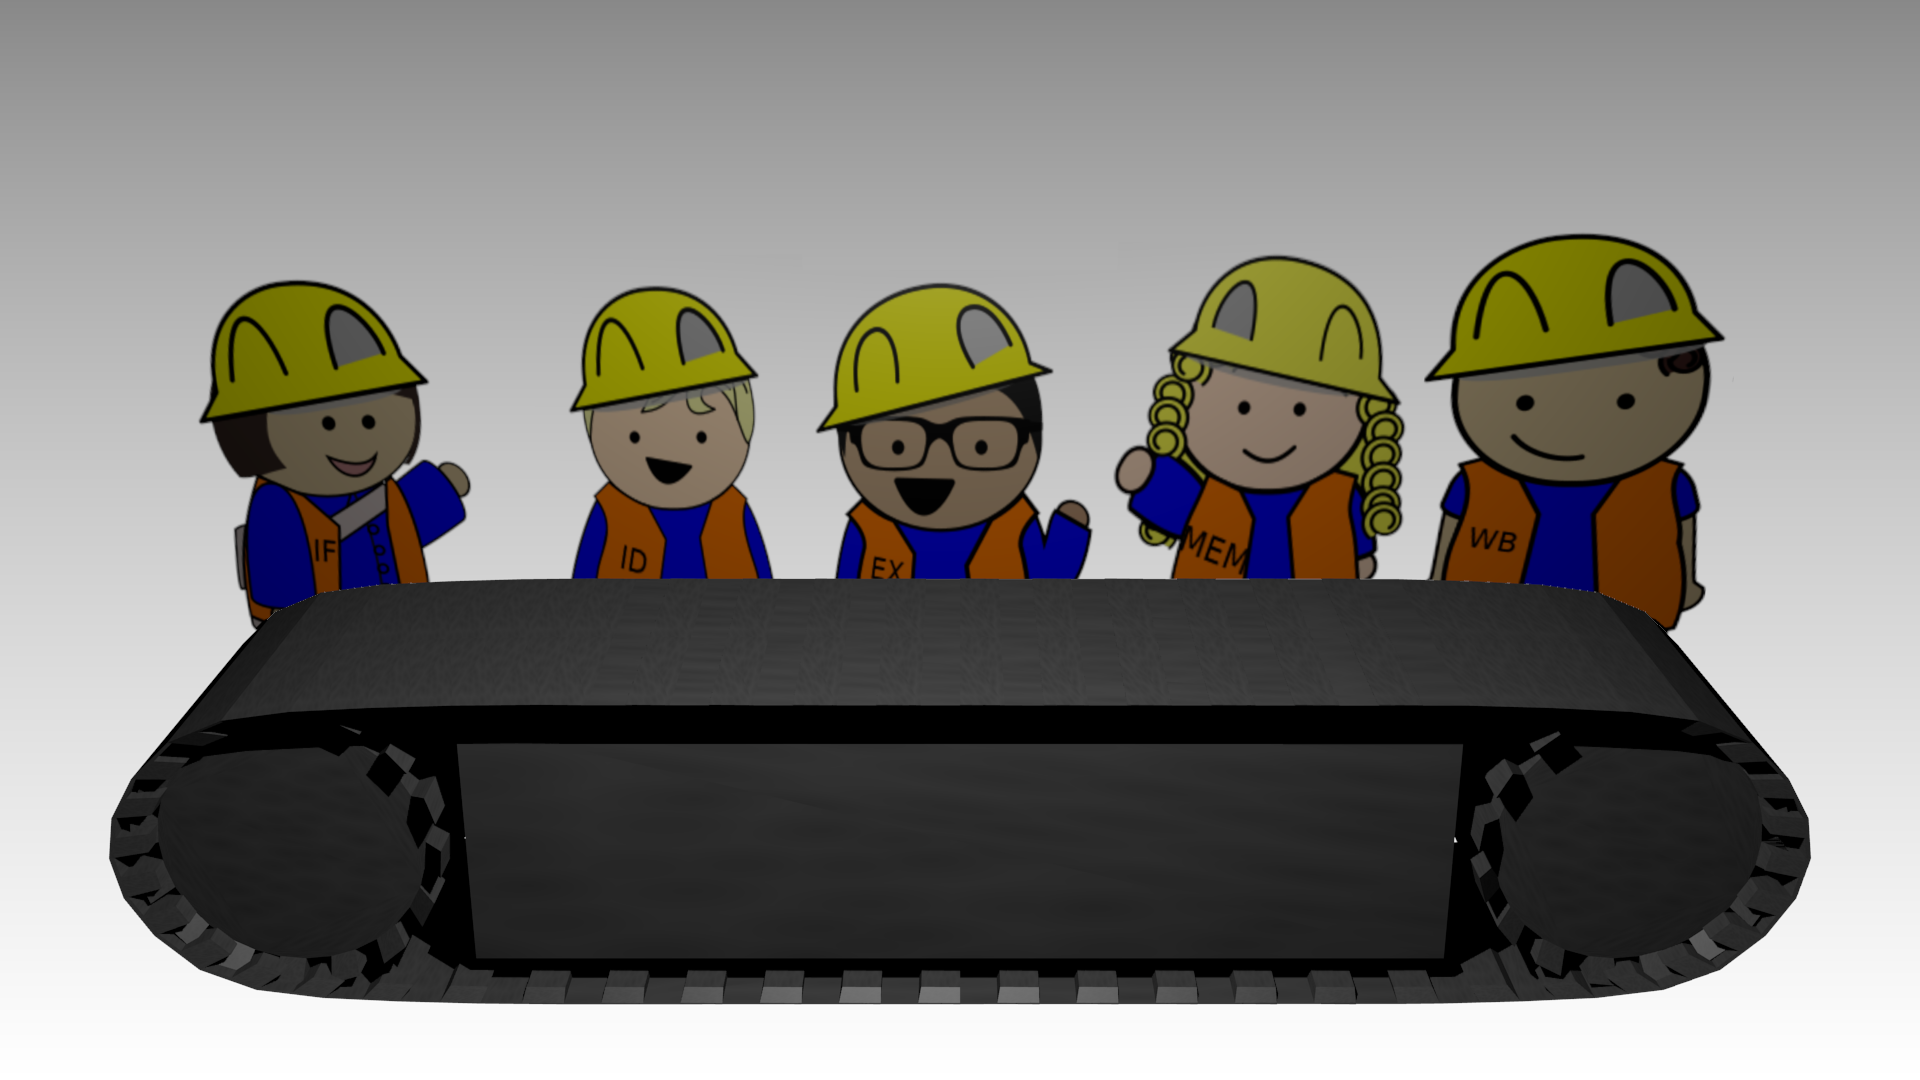
\includegraphics[width=1.0\textwidth]{final.png}}
%FETCH
\put(50,-12){\fontsize{5.5}{4}\selectfont\color{white}}

%DECODE
\put(90,-12){\fontsize{5.5}{4}\selectfont\color{white}}
\put(90,-17){\fontsize{5.5}{4}\selectfont\color{white}}

%EXECUTE
\put(135,-12){\fontsize{5.5}{4}\selectfont\color{white}mul t0, t1, t2}
\put(135,-17){\fontsize{5.5}{4}\selectfont\color{white}t0 = 1 * 3}
\put(135,-22){\fontsize{5.5}{4}\selectfont\color{white}t0 = 3}

%MEMORY
\put(185,-12){\fontsize{5.5}{4}\selectfont\color{white}add t4, zero, 5}
\put(185,-17){\fontsize{5.5}{4}\selectfont\color{white}t4 = 0 + 5}
\put(185,-22){\fontsize{5.5}{4}\selectfont\color{white}t4 = 5}

%WRITEBACK
\put(225,-12){\fontsize{5.5}{4}\selectfont\color{white}add t3, zero, 4}
\put(225,-17){\fontsize{5.5}{4}\selectfont\color{white}t3 = 0 + 4}
\put(225,-22){\fontsize{5.5}{4}\selectfont\color{white}t3 = 4}

%REGISTERS
\put(80,-37){\fontsize{5.5}{4}\selectfont\color{white}zero = 0}
\put(80,-42){\fontsize{5.5}{4}\selectfont\color{white}ra = 0}
\put(80,-47){\fontsize{5.5}{4}\selectfont\color{white}sp = 0}
\put(80,-52){\fontsize{5.5}{4}\selectfont\color{white}pc = 44}
\put(80,-57){\fontsize{5.5}{4}\selectfont\color{white}t0 = 1}
\put(80,-62){\fontsize{5.5}{4}\selectfont\color{white}t1 = 1}

\put(110,-37){\fontsize{5.5}{4}\selectfont\color{white}t2 = 3}
\put(110,-42){\fontsize{5.5}{4}\selectfont\color{white}t3 = 4}
\put(110,-47){\fontsize{5.5}{4}\selectfont\color{white}t4 = 0}
\put(110,-52){\fontsize{5.5}{4}\selectfont\color{white}t5 = 0}
\put(110,-57){\fontsize{5.5}{4}\selectfont\color{white}t6 = 0}
\put(110,-62){\fontsize{5.5}{4}\selectfont\color{white}a0 = 0}

\put(140,-37){\fontsize{5.5}{4}\selectfont\color{white}a1 = 0}
\put(140,-42){\fontsize{5.5}{4}\selectfont\color{white}a2 = 0}
\put(140,-47){\fontsize{5.5}{4}\selectfont\color{white}a3 = 0}
\put(140,-52){\fontsize{5.5}{4}\selectfont\color{white}a4 = 0}
\put(140,-57){\fontsize{5.5}{4}\selectfont\color{white}a5 = 0}
\put(140,-62){\fontsize{5.5}{4}\selectfont\color{white}a6 = 0}

\put(170,-37){\fontsize{5.5}{4}\selectfont\color{white}a7 = 0}
\put(170,-42){\fontsize{5.5}{4}\selectfont\color{white}s1 = 0}
\put(170,-47){\fontsize{5.5}{4}\selectfont\color{white}s2 = 0}
\put(170,-52){\fontsize{5.5}{4}\selectfont\color{white}s3 = 0}
\put(170,-57){\fontsize{5.5}{4}\selectfont\color{white}s4 = 0}
\put(170,-62){\fontsize{5.5}{4}\selectfont\color{white}s5 = 0}

\put(200,-37){\fontsize{5.5}{4}\selectfont\color{white}s6 = 0}
\put(200,-42){\fontsize{5.5}{4}\selectfont\color{white}s7 = 0}
\put(200,-47){\fontsize{5.5}{4}\selectfont\color{white}s8 = 0}
\put(200,-52){\fontsize{5.5}{4}\selectfont\color{white}s9 = 0}
\put(200,-57){\fontsize{5.5}{4}\selectfont\color{white}s10 = 0}
\put(200,-62){\fontsize{5.5}{4}\selectfont\color{white}s11 = 0}

\end{picture}
\end{frame}

\begin{frame}
\frametitle{Conditional Branch | Takt 11}
\begin{picture}(0,0)
\put(0,-85){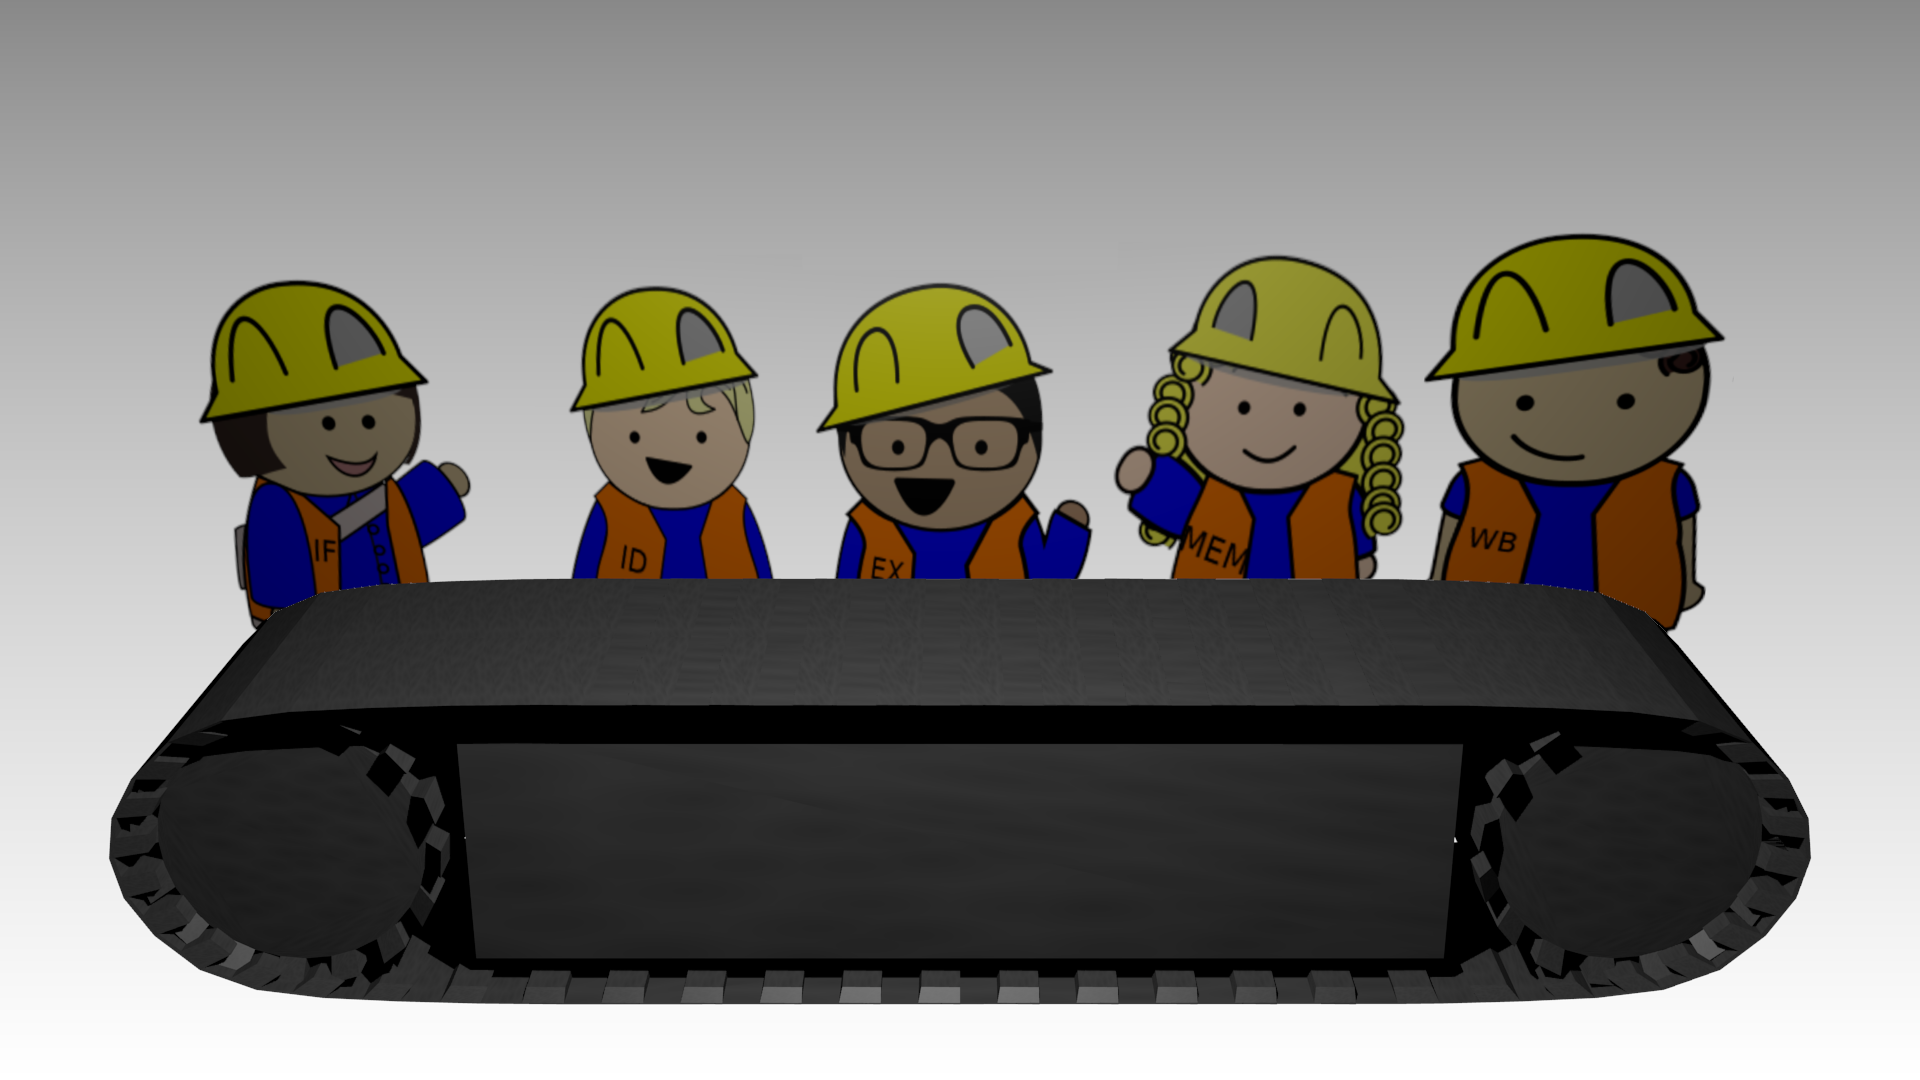
\includegraphics[width=1.0\textwidth]{final.png}}
%FETCH
\put(50,-12){\fontsize{5.5}{4}\selectfont\color{white}}

%DECODE
\put(90,-12){\fontsize{5.5}{4}\selectfont\color{white}}
\put(90,-17){\fontsize{5.5}{4}\selectfont\color{white}}

%EXECUTE
\put(135,-12){\fontsize{5.5}{4}\selectfont\color{white}}
\put(135,-17){\fontsize{5.5}{4}\selectfont\color{white}}
\put(135,-22){\fontsize{5.5}{4}\selectfont\color{white}}

%MEMORY
\put(185,-12){\fontsize{5.5}{4}\selectfont\color{white}mul t0, t1, t2}
\put(185,-17){\fontsize{5.5}{4}\selectfont\color{white}t0 = 1 * 3}
\put(185,-22){\fontsize{5.5}{4}\selectfont\color{white}t0 = 3}

%WRITEBACK
\put(225,-12){\fontsize{5.5}{4}\selectfont\color{white}add t4, zero, 5}
\put(225,-17){\fontsize{5.5}{4}\selectfont\color{white}t4 = 0 + 5}
\put(225,-22){\fontsize{5.5}{4}\selectfont\color{white}t4 = 5}

%REGISTERS
\put(80,-37){\fontsize{5.5}{4}\selectfont\color{white}zero = 0}
\put(80,-42){\fontsize{5.5}{4}\selectfont\color{white}ra = 0}
\put(80,-47){\fontsize{5.5}{4}\selectfont\color{white}sp = 0}
\put(80,-52){\fontsize{5.5}{4}\selectfont\color{white}pc = 48}
\put(80,-57){\fontsize{5.5}{4}\selectfont\color{white}t0 = 1}
\put(80,-62){\fontsize{5.5}{4}\selectfont\color{white}t1 = 1}

\put(110,-37){\fontsize{5.5}{4}\selectfont\color{white}t2 = 3}
\put(110,-42){\fontsize{5.5}{4}\selectfont\color{white}t3 = 4}
\put(110,-47){\fontsize{5.5}{4}\selectfont\color{white}t4 = 5}
\put(110,-52){\fontsize{5.5}{4}\selectfont\color{white}t5 = 0}
\put(110,-57){\fontsize{5.5}{4}\selectfont\color{white}t6 = 0}
\put(110,-62){\fontsize{5.5}{4}\selectfont\color{white}a0 = 0}

\put(140,-37){\fontsize{5.5}{4}\selectfont\color{white}a1 = 0}
\put(140,-42){\fontsize{5.5}{4}\selectfont\color{white}a2 = 0}
\put(140,-47){\fontsize{5.5}{4}\selectfont\color{white}a3 = 0}
\put(140,-52){\fontsize{5.5}{4}\selectfont\color{white}a4 = 0}
\put(140,-57){\fontsize{5.5}{4}\selectfont\color{white}a5 = 0}
\put(140,-62){\fontsize{5.5}{4}\selectfont\color{white}a6 = 0}

\put(170,-37){\fontsize{5.5}{4}\selectfont\color{white}a7 = 0}
\put(170,-42){\fontsize{5.5}{4}\selectfont\color{white}s1 = 0}
\put(170,-47){\fontsize{5.5}{4}\selectfont\color{white}s2 = 0}
\put(170,-52){\fontsize{5.5}{4}\selectfont\color{white}s3 = 0}
\put(170,-57){\fontsize{5.5}{4}\selectfont\color{white}s4 = 0}
\put(170,-62){\fontsize{5.5}{4}\selectfont\color{white}s5 = 0}

\put(200,-37){\fontsize{5.5}{4}\selectfont\color{white}s6 = 0}
\put(200,-42){\fontsize{5.5}{4}\selectfont\color{white}s7 = 0}
\put(200,-47){\fontsize{5.5}{4}\selectfont\color{white}s8 = 0}
\put(200,-52){\fontsize{5.5}{4}\selectfont\color{white}s9 = 0}
\put(200,-57){\fontsize{5.5}{4}\selectfont\color{white}s10 = 0}
\put(200,-62){\fontsize{5.5}{4}\selectfont\color{white}s11 = 0}

\end{picture}
\end{frame}


\begin{frame}
\frametitle{Conditional Branch | Takt 12}
\begin{picture}(0,0)
\put(0,-85){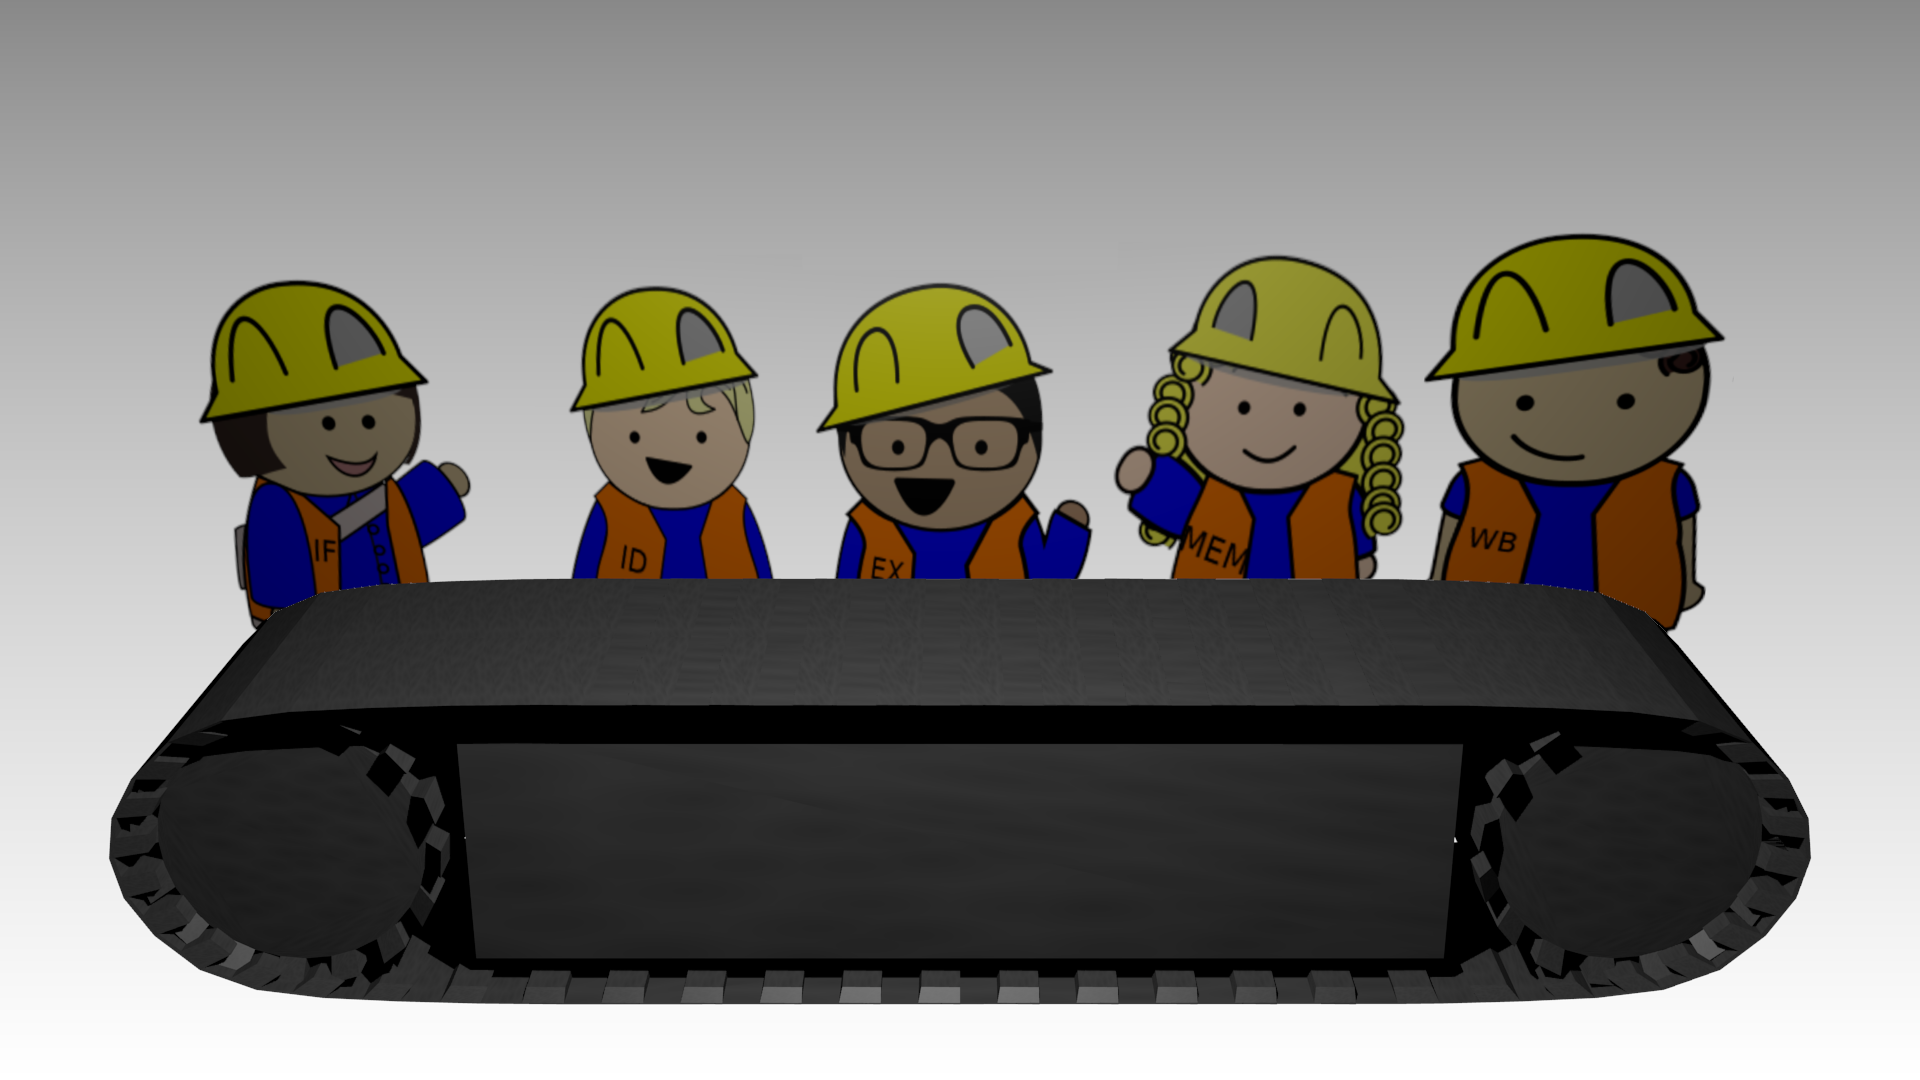
\includegraphics[width=1.0\textwidth]{final.png}}
%FETCH
\put(50,-12){\fontsize{5.5}{4}\selectfont\color{white}}

%DECODE
\put(90,-12){\fontsize{5.5}{4}\selectfont\color{white}}
\put(90,-17){\fontsize{5.5}{4}\selectfont\color{white}}

%EXECUTE
\put(135,-12){\fontsize{5.5}{4}\selectfont\color{white}}
\put(135,-17){\fontsize{5.5}{4}\selectfont\color{white}}
\put(135,-22){\fontsize{5.5}{4}\selectfont\color{white}}

%MEMORY
\put(185,-12){\fontsize{5.5}{4}\selectfont\color{white}}
\put(185,-17){\fontsize{5.5}{4}\selectfont\color{white}}
\put(185,-22){\fontsize{5.5}{4}\selectfont\color{white}}

%WRITEBACK
\put(225,-12){\fontsize{5.5}{4}\selectfont\color{white}mul t0, t1, t2}
\put(225,-17){\fontsize{5.5}{4}\selectfont\color{white}t0 = 1 * 3}
\put(225,-22){\fontsize{5.5}{4}\selectfont\color{white}t0 = 3}

%REGISTERS
\put(80,-37){\fontsize{5.5}{4}\selectfont\color{white}zero = 0}
\put(80,-42){\fontsize{5.5}{4}\selectfont\color{white}ra = 0}
\put(80,-47){\fontsize{5.5}{4}\selectfont\color{white}sp = 0}
\put(80,-52){\fontsize{5.5}{4}\selectfont\color{white}pc = 52}
\put(80,-57){\fontsize{5.5}{4}\selectfont\color{white}t0 = 3}
\put(80,-62){\fontsize{5.5}{4}\selectfont\color{white}t1 = 1}

\put(110,-37){\fontsize{5.5}{4}\selectfont\color{white}t2 = 3}
\put(110,-42){\fontsize{5.5}{4}\selectfont\color{white}t3 = 4}
\put(110,-47){\fontsize{5.5}{4}\selectfont\color{white}t4 = 5}
\put(110,-52){\fontsize{5.5}{4}\selectfont\color{white}t5 = 0}
\put(110,-57){\fontsize{5.5}{4}\selectfont\color{white}t6 = 0}
\put(110,-62){\fontsize{5.5}{4}\selectfont\color{white}a0 = 0}

\put(140,-37){\fontsize{5.5}{4}\selectfont\color{white}a1 = 0}
\put(140,-42){\fontsize{5.5}{4}\selectfont\color{white}a2 = 0}
\put(140,-47){\fontsize{5.5}{4}\selectfont\color{white}a3 = 0}
\put(140,-52){\fontsize{5.5}{4}\selectfont\color{white}a4 = 0}
\put(140,-57){\fontsize{5.5}{4}\selectfont\color{white}a5 = 0}
\put(140,-62){\fontsize{5.5}{4}\selectfont\color{white}a6 = 0}

\put(170,-37){\fontsize{5.5}{4}\selectfont\color{white}a7 = 0}
\put(170,-42){\fontsize{5.5}{4}\selectfont\color{white}s1 = 0}
\put(170,-47){\fontsize{5.5}{4}\selectfont\color{white}s2 = 0}
\put(170,-52){\fontsize{5.5}{4}\selectfont\color{white}s3 = 0}
\put(170,-57){\fontsize{5.5}{4}\selectfont\color{white}s4 = 0}
\put(170,-62){\fontsize{5.5}{4}\selectfont\color{white}s5 = 0}

\put(200,-37){\fontsize{5.5}{4}\selectfont\color{white}s6 = 0}
\put(200,-42){\fontsize{5.5}{4}\selectfont\color{white}s7 = 0}
\put(200,-47){\fontsize{5.5}{4}\selectfont\color{white}s8 = 0}
\put(200,-52){\fontsize{5.5}{4}\selectfont\color{white}s9 = 0}
\put(200,-57){\fontsize{5.5}{4}\selectfont\color{white}s10 = 0}
\put(200,-62){\fontsize{5.5}{4}\selectfont\color{white}s11 = 0}

\end{picture}
\end{frame}

\begin{frame}
\frametitle{Conditional Branch | Takt 13}
\begin{picture}(0,0)
\put(0,-85){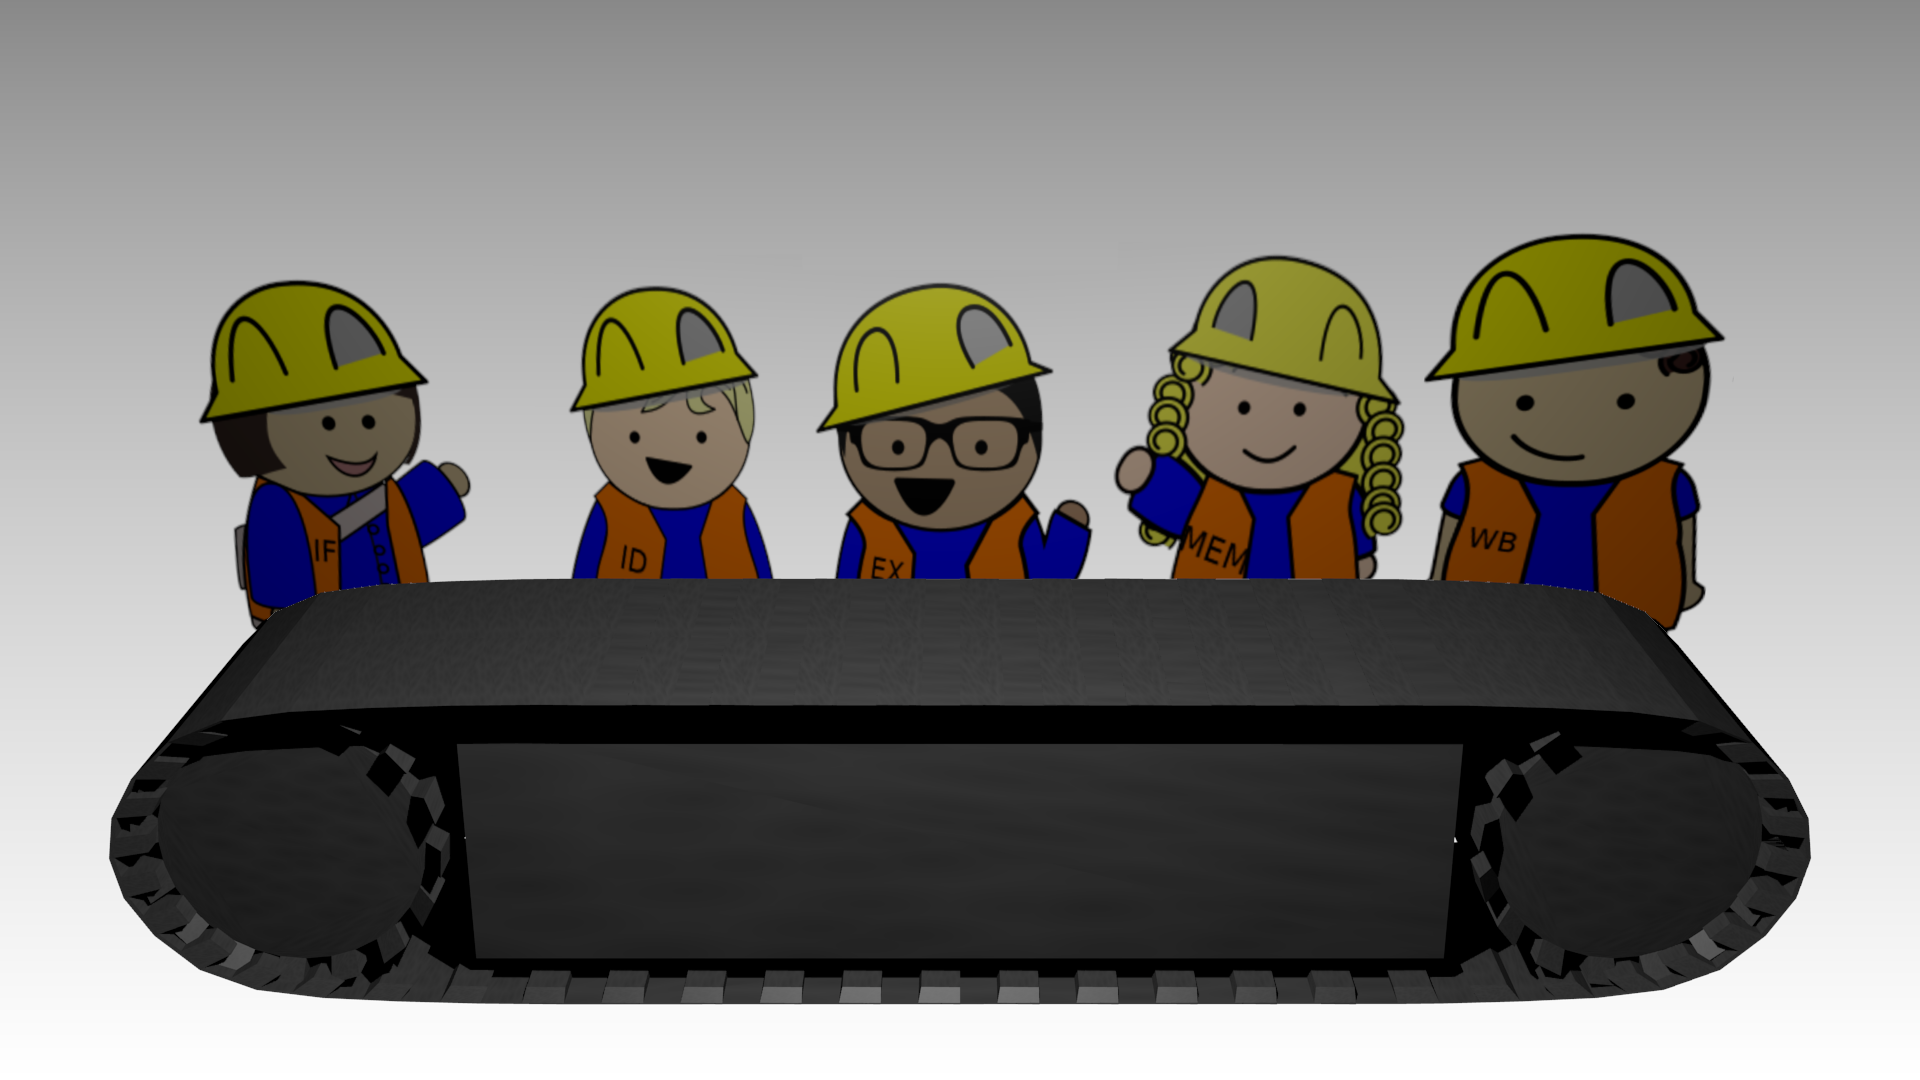
\includegraphics[width=1.0\textwidth]{final.png}}
%FETCH
\put(50,-12){\fontsize{5.5}{4}\selectfont\color{white}}

%DECODE
\put(90,-12){\fontsize{5.5}{4}\selectfont\color{white}}
\put(90,-17){\fontsize{5.5}{4}\selectfont\color{white}}

%EXECUTE
\put(135,-12){\fontsize{5.5}{4}\selectfont\color{white}}
\put(135,-17){\fontsize{5.5}{4}\selectfont\color{white}}
\put(135,-22){\fontsize{5.5}{4}\selectfont\color{white}}

%MEMORY
\put(185,-12){\fontsize{5.5}{4}\selectfont\color{white}}
\put(185,-17){\fontsize{5.5}{4}\selectfont\color{white}}
\put(185,-22){\fontsize{5.5}{4}\selectfont\color{white}}

%WRITEBACK
\put(225,-12){\fontsize{5.5}{4}\selectfont\color{white}}
\put(225,-17){\fontsize{5.5}{4}\selectfont\color{white}}
\put(225,-22){\fontsize{5.5}{4}\selectfont\color{white}}

%REGISTERS
\put(80,-37){\fontsize{5.5}{4}\selectfont\color{white}zero = 0}
\put(80,-42){\fontsize{5.5}{4}\selectfont\color{white}ra = 0}
\put(80,-47){\fontsize{5.5}{4}\selectfont\color{white}sp = 0}
\put(80,-52){\fontsize{5.5}{4}\selectfont\color{white}pc = 56}
\put(80,-57){\fontsize{5.5}{4}\selectfont\color{white}t0 = 3}
\put(80,-62){\fontsize{5.5}{4}\selectfont\color{white}t1 = 1}

\put(110,-37){\fontsize{5.5}{4}\selectfont\color{white}t2 = 3}
\put(110,-42){\fontsize{5.5}{4}\selectfont\color{white}t3 = 4}
\put(110,-47){\fontsize{5.5}{4}\selectfont\color{white}t4 = 5}
\put(110,-52){\fontsize{5.5}{4}\selectfont\color{white}t5 = 0}
\put(110,-57){\fontsize{5.5}{4}\selectfont\color{white}t6 = 0}
\put(110,-62){\fontsize{5.5}{4}\selectfont\color{white}a0 = 0}

\put(140,-37){\fontsize{5.5}{4}\selectfont\color{white}a1 = 0}
\put(140,-42){\fontsize{5.5}{4}\selectfont\color{white}a2 = 0}
\put(140,-47){\fontsize{5.5}{4}\selectfont\color{white}a3 = 0}
\put(140,-52){\fontsize{5.5}{4}\selectfont\color{white}a4 = 0}
\put(140,-57){\fontsize{5.5}{4}\selectfont\color{white}a5 = 0}
\put(140,-62){\fontsize{5.5}{4}\selectfont\color{white}a6 = 0}

\put(170,-37){\fontsize{5.5}{4}\selectfont\color{white}a7 = 0}
\put(170,-42){\fontsize{5.5}{4}\selectfont\color{white}s1 = 0}
\put(170,-47){\fontsize{5.5}{4}\selectfont\color{white}s2 = 0}
\put(170,-52){\fontsize{5.5}{4}\selectfont\color{white}s3 = 0}
\put(170,-57){\fontsize{5.5}{4}\selectfont\color{white}s4 = 0}
\put(170,-62){\fontsize{5.5}{4}\selectfont\color{white}s5 = 0}

\put(200,-37){\fontsize{5.5}{4}\selectfont\color{white}s6 = 0}
\put(200,-42){\fontsize{5.5}{4}\selectfont\color{white}s7 = 0}
\put(200,-47){\fontsize{5.5}{4}\selectfont\color{white}s8 = 0}
\put(200,-52){\fontsize{5.5}{4}\selectfont\color{white}s9 = 0}
\put(200,-57){\fontsize{5.5}{4}\selectfont\color{white}s10 = 0}
\put(200,-62){\fontsize{5.5}{4}\selectfont\color{white}s11 = 0}

\end{picture}
\end{frame}

\end{document}

%%%%%%%%%%%%%%%%%%%%%%%%%%%%%%%%%%%%%%%%%%%%%%%%%%%%%%%%%%%%%%%%%%%%%%%%%%%%%%%
